\documentclass[oneside, notitlepage]{book}
%\documentclass[twoside]{article} %---original command 


\documentclass[twoside]{article} %---original command 

% the preamble which specifies packages and parameters for the document
\usepackage{graphics}
\usepackage[pdftex]{color,graphicx}
\usepackage{amsthm}
\usepackage{relsize}
\usepackage{amsmath}
\usepackage{amssymb}
\usepackage{framed}

% for inserting URL's into a page
\usepackage[colorlinks=true]{hyperref}

% for numbering lists with (a) (b) (c) and other such nice things
\usepackage[inline]{enumitem}
% optional [inline] option is to get the enumerate* environment (or *enumerate; something like that)

% for blackboard 1's to use with indicator functions
\usepackage{bbold}

%	adds script font, useful e.g. for defining normal RV's or sigma-algebras, \mathscr
\usepackage{mathrsfs}

%----we require the package mathtools in order for the following
%DeclaredPairedDelimiter thing to work, e.g. absolute value and norm
\usepackage{mathtools}
% We also require mathtools for \shortintertext to work

%---required for the commands in the formatting preamble:
\usepackage{fancyhdr}

%-------------Discussion of reasons for using this pacakge can be found here: https://tex.stackexchange.com/questions/29973/more-than-one-optional-argument-for-newcommand or here: https://tex.stackexchange.com/questions/145175/optional-arguments-xparse-vs-xargs  ----------
\usepackage{xargs}
%---------------------Long term, using xparse might be a better implementation
%---use it for the headers and footers commands

%---needed for the custom block quote things. the most argument is as recommended in the answers here:
%--- https://tex.stackexchange.com/a/238296/103825   and  here:  https://tex.stackexchange.com/a/265804/103825
\usepackage[most]{tcolorbox}


% https://tex.stackexchange.com/questions/3238/bm-package-versus-boldsymbol
% This answer says this has to be loaded after all font packages to work correctly: https://tex.stackexchange.com/a/179337
\usepackage{bm}






%---says not to indent paragraphs
\setlength{\parindent}{0 in}

%---set up headers and footers for pages further into the document:

% \headerfooter{Course }[optional:  assignment type]{ number of problem set }{ due date }[your name]
\newcommandx{\headerfooter}[5][2={}, 5={} ]{
\pagestyle{fancy}
\lhead{#2 #3}
\rhead{#4}
\chead{}
\lfoot{#5}
\cfoot{#1}
\rfoot{Page \thepage}

}
%---uses the package fancyhdr
%---also uses package xargs for the newcommandx with the optional parameters


%---uses the package tcolorbox
%---follows exactly answers here: https://tex.stackexchange.com/a/265804/103825 and here: https://tex.stackexchange.com/a/238296/103825 except that environment name is different
\definecolor{block-gray}{gray}{0.85}
\newtcolorbox{blockquote}{colback=block-gray,grow to right by=-10mm,grow to left by=-10mm,
boxrule=0pt,boxsep=0pt,breakable}
%--- see the documentation for explanation of all of the parameter values: https://mirror.hmc.edu/ctan/macros/latex/contrib/tcolorbox/tcolorbox.pdf

% The following macro is used to generate a general header

% \frontbox{ Class/Course }{ type of document }{ number of document type }{ date }[your name][Thing to add before date]
\newcommandx{\frontbox}[6][ 5={William Krinsman}, 6={} ]{
	%----------------- Note how we have to use \newcommandx  (emphasis on the X) instead of \newcommand in order to access the functionality of the xargs package
   \newpage
   \noindent

   \begin{blockquote}
        {#1 \hfill Spring 2018 }

       \vspace{4mm}

       % Add in the number of the assignment
       { {\Huge \hfill #2 #3  \hfill} }

        \vspace{4mm}
       % Add in the specific due date of the problem set as well as your name
       { { #5 \hfill #6 #4} }

   \end{blockquote}


}


%%% Local Variables:
%%% mode: latex
%%% TeX-master: "../report/LaTeX-files/main/report"
%%% End:

%			New math operators

%new, specialized math commands:
%----argmin
\DeclareMathOperator*{\argmin}{\arg\!\min}
%----argmax
\DeclareMathOperator*{\argmax}{\arg\!\max}
%----partial derivatives
\newcommand{\partialderivative}[2][]{\frac{ \partial #1   }{ \partial #2  } }

%----note 1: the following commands require mathtools package
%----note: the DeclarePairedDelimiter and thus the mathtools package are helpful because of this: https://tex.stackexchange.com/questions/2607/spacing-around-left-and-right

%----absolute value
\DeclarePairedDelimiter\absolutevalue{\lvert}{\rvert}
%----norm
\DeclarePairedDelimiter\norm{\lVert}{\rVert}
%----floor
\DeclarePairedDelimiter\floor{\lfloor}{\rfloor}


%			Commonly used symbols

%	real numbers
\newcommand{\reals}{\mathbb{R}}
%	natural numbers
\newcommand{\naturals}{\mathbb{N}}
%	integers
\newcommand{\integers}{\mathbb{Z}}
% 	switches the default epsilon to be the good epsilon and the backup epsilon to be the bad epsilon
\let\otherepsilon\epsilon
\let\realepsilon\varepsilon
\let\varepsilon\otherepsilon
\let\epsilon\realepsilon
% independence sign -- don't quite understand how works, but see here: https://tex.stackexchange.com/questions/79434/double-perpendicular-symbol-for-independence
\newcommand\independent{\protect\mathpalette{\protect\independenT}{\perp}}
\def\independenT#1#2{\mathrel{\rlap{$#1#2$}\mkern6mu{#1#2}}}


% 			Probability Theory

%	expectation operator
\newcommand{\expectation}{\mathbb{E}}
%	probability measure
\newcommand{\probability}{\mathbb{P}}
% indicator functions.  NOTE: this requires package bbold for \mathbb{1} to work
\newcommand{\indicator}[1]{\mathbb{1}_{#1}}
% Variance
\newcommand{\variance}{\operatorname{Var}}
% Covariance
\newcommand{\covariance}{\operatorname{Cov}}
% independent and identically distributed
\newcommand{\iid}{\overset{i.i.d.}{\sim}}

%			Equation formatting

%	simplified procedure for creating (square bracket shaped) matrices
\newcommand{\Matrix}[1]{  \begin{bmatrix}  #1  \end{bmatrix}  }

%	simplified procedure for putting expressions into parentheses
\newcommand{\parentheses}[1]{  \left(   #1  \right)   }
%	simplified procedure for putting expressions into square brackets
\newcommand{\brackets}[1]{  \left[   #1  \right]   }

% 	load the array package, required for solution given below for equation formatting, see here: https://tex.stackexchange.com/questions/44407/make-every-element-of-an-array-displaystyle
\usepackage{array}
%    also  loading the longtable package for allowing page breaks, see here: https://tex.stackexchange.com/questions/317121/automatically-adding-page-breaks-into-long-array-environments
% did not actually work, it just messed everything up, because interpreter doesn't think longtable is math mode or whatever
% apparently longtable is not designed to be math mode? https://tex.stackexchange.com/questions/155298/math-mode-in-longtabu
% so if I want to use longtable instead of array here, it would require more than just replacing ``array'' with  ``longtable''.


%	waste less time setting up the formatting for equations
\newenvironment{formulae} [1] [3] {
	
	% See array package documentation: http://mirrors.rit.edu/CTAN/macros/latex/required/tools/array.pdf
	% creates three new column types, which are just the regular column types, but with displaystyle inserted automatically before each entry
	\newcolumntype{C}{>{\displaystyle}c}
	\newcolumntype{L}{>{\displaystyle}l}
	\newcolumntype{R}{>{\displaystyle}r}

        % See answer here: https://tex.stackexchange.com/a/267485
       \begingroup\abovedisplayskip=-6pt \abovedisplayshortskip=-6pt \belowdisplayshortskip=-3pt \belowdisplayskip=-3pt
       % https://tex.stackexchange.com/questions/51682/is-it-possible-to-pagebreak-aligned-equations
       %\allowdisplaybreaks
       % above (allowdisplaybreaks) doesn't work though because supposedly only works for the environments from amsmath package unfortunately

	\[  \begin{array}{R*{\numexpr #1 -2}CL<{\smallskip \smallskip}} 
 }{	
 
 % according to here, the size of smallskip (\smallskipamount) is 3.0 pt each, https://tex.stackexchange.com/questions/114569/space-between-paragraphs-local
 % so to delete two unnecessary smallskips after the end of one of these environments arrays, all we have to do is delete 6pt so that is what is now done before ending the array
\\[-6pt]


	\end{array} \]	

\endgroup
 }

% copy-pasted from here: https://tex.stackexchange.com/questions/280819/vertical-space-command-which-is-between-intertext-and-shortintertext
\MHInternalSyntaxOn
\newcommandx{\adjintertext} [3] [1={-15pt}, 2={3pt}]% #1=above skip, #2=below skip, #3=text
{\ifvmode\else\\\@empty\fi
  \noalign{%
    %\penalty\postdisplaypenalty\vskip\belowdisplayskip
    \vskip-\lineskiplimit      % CCS
    \vskip\normallineskiplimit % CCS
    \vskip#1
     \vbox{\normalbaselines
       \ifdim
         \ifdim\@totalleftmargin=\z@
           \linewidth
         \else
           -\maxdimen
         \fi
       =\columnwidth
      \else \parshape\@ne \@totalleftmargin \linewidth
      \fi
      \noindent#3\par}%
    %\penalty\predisplaypenalty\vskip\abovedisplayskip%
    \vskip-\lineskiplimit      % CCS
    \vskip\normallineskiplimit % CCS
    \vskip#2
 }}%
\MHInternalSyntaxOff



    
    
    \usepackage[T1]{fontenc}
    % Nicer default font (+ math font) than Computer Modern for most use cases
    \usepackage{mathpazo}


    % We will generate all images so they have a width \maxwidth. This means
    % that they will get their normal width if they fit onto the page, but
    % are scaled down if they would overflow the margins.
    \makeatletter
    \def\maxwidth{\ifdim\Gin@nat@width>\linewidth\linewidth
    \else\Gin@nat@width\fi}
    \makeatother
    \let\Oldincludegraphics\includegraphics
    % Set max figure width to be 80% of text width, for now hardcoded.
    \renewcommand{\includegraphics}[1]{\Oldincludegraphics[width=.8\maxwidth]{#1}}
    % Ensure that by default, figures have no caption (until we provide a
    % proper Figure object with a Caption API and a way to capture that
    % in the conversion process - todo).
    \usepackage{caption}
    \DeclareCaptionLabelFormat{nolabel}{}
    \captionsetup{labelformat=nolabel}

    \usepackage{adjustbox} % Used to constrain images to a maximum size 
    \usepackage{xcolor} % Allow colors to be defined
    \usepackage{geometry} % Used to adjust the document margins
    \usepackage{textcomp} % defines textquotesingle
    % Hack from http://tex.stackexchange.com/a/47451/13684:
    \AtBeginDocument{%
        \def\PYZsq{\textquotesingle}% Upright quotes in Pygmentized code
    }
    \usepackage{upquote} % Upright quotes for verbatim code
    \usepackage{eurosym} % defines \euro

    % apparently ucs is incompatible with biblatex? so commented out
    %\usepackage[mathletters]{ucs} % Extended unicode (utf-8) support

    % according to here: https://tex.stackexchange.com/questions/215654/biblatex-package-problem#comment506283_215654
    \usepackage[utf8]{inputenc} % Allow utf-8 characters in the tex document
    % the original option, utf8x, chosen by Jupyter notebook stealthily imports ucs -- we don't want that b/c biblatex complains so it's been changed

    \usepackage{fancyvrb} % verbatim replacement that allows latex
    \usepackage{grffile} % extends the file name processing of package graphics 
                         % to support a larger range 
    % The hyperref package gives us a pdf with properly built
    % internal navigation ('pdf bookmarks' for the table of contents,
    % internal cross-reference links, web links for URLs, etc.)

    \usepackage{longtable} % longtable support required by pandoc >1.10
    % according to answer here: https://tex.stackexchange.com/questions/32726/center-wide-longtable-not-tabular-or-tabularx/32729
    % can be used to avoid the table being too far in the center
    \setlength{\LTleft}{-1cm plus -1fill}

    \usepackage{booktabs}  % table support for pandoc > 1.12.2
    \usepackage[normalem]{ulem} % ulem is needed to support strikethroughs (\sout)
                                % normalem makes italics be italics, not underlines
    

    
    
    % Colors for the hyperref package
    \definecolor{urlcolor}{rgb}{0,.145,.698}
    \definecolor{linkcolor}{rgb}{.71,0.21,0.01}
    \definecolor{citecolor}{rgb}{.12,.54,.11}

    % ANSI colors
    \definecolor{ansi-black}{HTML}{3E424D}
    \definecolor{ansi-black-intense}{HTML}{282C36}
    \definecolor{ansi-red}{HTML}{E75C58}
    \definecolor{ansi-red-intense}{HTML}{B22B31}
    \definecolor{ansi-green}{HTML}{00A250}
    \definecolor{ansi-green-intense}{HTML}{007427}
    \definecolor{ansi-yellow}{HTML}{DDB62B}
    \definecolor{ansi-yellow-intense}{HTML}{B27D12}
    \definecolor{ansi-blue}{HTML}{208FFB}
    \definecolor{ansi-blue-intense}{HTML}{0065CA}
    \definecolor{ansi-magenta}{HTML}{D160C4}
    \definecolor{ansi-magenta-intense}{HTML}{A03196}
    \definecolor{ansi-cyan}{HTML}{60C6C8}
    \definecolor{ansi-cyan-intense}{HTML}{258F8F}
    \definecolor{ansi-white}{HTML}{C5C1B4}
    \definecolor{ansi-white-intense}{HTML}{A1A6B2}

    % commands and environments needed by pandoc snippets
    % extracted from the output of `pandoc -s`
    \providecommand{\tightlist}{%
      \setlength{\itemsep}{0pt}\setlength{\parskip}{0pt}}
    \DefineVerbatimEnvironment{Highlighting}{Verbatim}{commandchars=\\\{\}}
    % Add ',fontsize=\small' for more characters per line
    \newenvironment{Shaded}{}{}
    \newcommand{\KeywordTok}[1]{\textcolor[rgb]{0.00,0.44,0.13}{\textbf{{#1}}}}
    \newcommand{\DataTypeTok}[1]{\textcolor[rgb]{0.56,0.13,0.00}{{#1}}}
    \newcommand{\DecValTok}[1]{\textcolor[rgb]{0.25,0.63,0.44}{{#1}}}
    \newcommand{\BaseNTok}[1]{\textcolor[rgb]{0.25,0.63,0.44}{{#1}}}
    \newcommand{\FloatTok}[1]{\textcolor[rgb]{0.25,0.63,0.44}{{#1}}}
    \newcommand{\CharTok}[1]{\textcolor[rgb]{0.25,0.44,0.63}{{#1}}}
    \newcommand{\StringTok}[1]{\textcolor[rgb]{0.25,0.44,0.63}{{#1}}}
    \newcommand{\CommentTok}[1]{\textcolor[rgb]{0.38,0.63,0.69}{\textit{{#1}}}}
    \newcommand{\OtherTok}[1]{\textcolor[rgb]{0.00,0.44,0.13}{{#1}}}
    \newcommand{\AlertTok}[1]{\textcolor[rgb]{1.00,0.00,0.00}{\textbf{{#1}}}}
    \newcommand{\FunctionTok}[1]{\textcolor[rgb]{0.02,0.16,0.49}{{#1}}}
    \newcommand{\RegionMarkerTok}[1]{{#1}}
    \newcommand{\ErrorTok}[1]{\textcolor[rgb]{1.00,0.00,0.00}{\textbf{{#1}}}}
    \newcommand{\NormalTok}[1]{{#1}}
    
    % Additional commands for more recent versions of Pandoc
    \newcommand{\ConstantTok}[1]{\textcolor[rgb]{0.53,0.00,0.00}{{#1}}}
    \newcommand{\SpecialCharTok}[1]{\textcolor[rgb]{0.25,0.44,0.63}{{#1}}}
    \newcommand{\VerbatimStringTok}[1]{\textcolor[rgb]{0.25,0.44,0.63}{{#1}}}
    \newcommand{\SpecialStringTok}[1]{\textcolor[rgb]{0.73,0.40,0.53}{{#1}}}
    \newcommand{\ImportTok}[1]{{#1}}
    \newcommand{\DocumentationTok}[1]{\textcolor[rgb]{0.73,0.13,0.13}{\textit{{#1}}}}
    \newcommand{\AnnotationTok}[1]{\textcolor[rgb]{0.38,0.63,0.69}{\textbf{\textit{{#1}}}}}
    \newcommand{\CommentVarTok}[1]{\textcolor[rgb]{0.38,0.63,0.69}{\textbf{\textit{{#1}}}}}
    \newcommand{\VariableTok}[1]{\textcolor[rgb]{0.10,0.09,0.49}{{#1}}}
    \newcommand{\ControlFlowTok}[1]{\textcolor[rgb]{0.00,0.44,0.13}{\textbf{{#1}}}}
    \newcommand{\OperatorTok}[1]{\textcolor[rgb]{0.40,0.40,0.40}{{#1}}}
    \newcommand{\BuiltInTok}[1]{{#1}}
    \newcommand{\ExtensionTok}[1]{{#1}}
    \newcommand{\PreprocessorTok}[1]{\textcolor[rgb]{0.74,0.48,0.00}{{#1}}}
    \newcommand{\AttributeTok}[1]{\textcolor[rgb]{0.49,0.56,0.16}{{#1}}}
    \newcommand{\InformationTok}[1]{\textcolor[rgb]{0.38,0.63,0.69}{\textbf{\textit{{#1}}}}}
    \newcommand{\WarningTok}[1]{\textcolor[rgb]{0.38,0.63,0.69}{\textbf{\textit{{#1}}}}}
    
    
    % Define a nice break command that doesn't care if a line doesn't already
    % exist.
    \def\br{\hspace*{\fill} \\* }
    % Math Jax compatability definitions
    \def\gt{>}
    \def\lt{<}

    
    
    

    % Pygments definitions
    
\makeatletter
\def\PY@reset{\let\PY@it=\relax \let\PY@bf=\relax%
    \let\PY@ul=\relax \let\PY@tc=\relax%
    \let\PY@bc=\relax \let\PY@ff=\relax}
\def\PY@tok#1{\csname PY@tok@#1\endcsname}
\def\PY@toks#1+{\ifx\relax#1\empty\else%
    \PY@tok{#1}\expandafter\PY@toks\fi}
\def\PY@do#1{\PY@bc{\PY@tc{\PY@ul{%
    \PY@it{\PY@bf{\PY@ff{#1}}}}}}}
\def\PY#1#2{\PY@reset\PY@toks#1+\relax+\PY@do{#2}}

\expandafter\def\csname PY@tok@w\endcsname{\def\PY@tc##1{\textcolor[rgb]{0.73,0.73,0.73}{##1}}}
\expandafter\def\csname PY@tok@c\endcsname{\let\PY@it=\textit\def\PY@tc##1{\textcolor[rgb]{0.25,0.50,0.50}{##1}}}
\expandafter\def\csname PY@tok@cp\endcsname{\def\PY@tc##1{\textcolor[rgb]{0.74,0.48,0.00}{##1}}}
\expandafter\def\csname PY@tok@k\endcsname{\let\PY@bf=\textbf\def\PY@tc##1{\textcolor[rgb]{0.00,0.50,0.00}{##1}}}
\expandafter\def\csname PY@tok@kp\endcsname{\def\PY@tc##1{\textcolor[rgb]{0.00,0.50,0.00}{##1}}}
\expandafter\def\csname PY@tok@kt\endcsname{\def\PY@tc##1{\textcolor[rgb]{0.69,0.00,0.25}{##1}}}
\expandafter\def\csname PY@tok@o\endcsname{\def\PY@tc##1{\textcolor[rgb]{0.40,0.40,0.40}{##1}}}
\expandafter\def\csname PY@tok@ow\endcsname{\let\PY@bf=\textbf\def\PY@tc##1{\textcolor[rgb]{0.67,0.13,1.00}{##1}}}
\expandafter\def\csname PY@tok@nb\endcsname{\def\PY@tc##1{\textcolor[rgb]{0.00,0.50,0.00}{##1}}}
\expandafter\def\csname PY@tok@nf\endcsname{\def\PY@tc##1{\textcolor[rgb]{0.00,0.00,1.00}{##1}}}
\expandafter\def\csname PY@tok@nc\endcsname{\let\PY@bf=\textbf\def\PY@tc##1{\textcolor[rgb]{0.00,0.00,1.00}{##1}}}
\expandafter\def\csname PY@tok@nn\endcsname{\let\PY@bf=\textbf\def\PY@tc##1{\textcolor[rgb]{0.00,0.00,1.00}{##1}}}
\expandafter\def\csname PY@tok@ne\endcsname{\let\PY@bf=\textbf\def\PY@tc##1{\textcolor[rgb]{0.82,0.25,0.23}{##1}}}
\expandafter\def\csname PY@tok@nv\endcsname{\def\PY@tc##1{\textcolor[rgb]{0.10,0.09,0.49}{##1}}}
\expandafter\def\csname PY@tok@no\endcsname{\def\PY@tc##1{\textcolor[rgb]{0.53,0.00,0.00}{##1}}}
\expandafter\def\csname PY@tok@nl\endcsname{\def\PY@tc##1{\textcolor[rgb]{0.63,0.63,0.00}{##1}}}
\expandafter\def\csname PY@tok@ni\endcsname{\let\PY@bf=\textbf\def\PY@tc##1{\textcolor[rgb]{0.60,0.60,0.60}{##1}}}
\expandafter\def\csname PY@tok@na\endcsname{\def\PY@tc##1{\textcolor[rgb]{0.49,0.56,0.16}{##1}}}
\expandafter\def\csname PY@tok@nt\endcsname{\let\PY@bf=\textbf\def\PY@tc##1{\textcolor[rgb]{0.00,0.50,0.00}{##1}}}
\expandafter\def\csname PY@tok@nd\endcsname{\def\PY@tc##1{\textcolor[rgb]{0.67,0.13,1.00}{##1}}}
\expandafter\def\csname PY@tok@s\endcsname{\def\PY@tc##1{\textcolor[rgb]{0.73,0.13,0.13}{##1}}}
\expandafter\def\csname PY@tok@sd\endcsname{\let\PY@it=\textit\def\PY@tc##1{\textcolor[rgb]{0.73,0.13,0.13}{##1}}}
\expandafter\def\csname PY@tok@si\endcsname{\let\PY@bf=\textbf\def\PY@tc##1{\textcolor[rgb]{0.73,0.40,0.53}{##1}}}
\expandafter\def\csname PY@tok@se\endcsname{\let\PY@bf=\textbf\def\PY@tc##1{\textcolor[rgb]{0.73,0.40,0.13}{##1}}}
\expandafter\def\csname PY@tok@sr\endcsname{\def\PY@tc##1{\textcolor[rgb]{0.73,0.40,0.53}{##1}}}
\expandafter\def\csname PY@tok@ss\endcsname{\def\PY@tc##1{\textcolor[rgb]{0.10,0.09,0.49}{##1}}}
\expandafter\def\csname PY@tok@sx\endcsname{\def\PY@tc##1{\textcolor[rgb]{0.00,0.50,0.00}{##1}}}
\expandafter\def\csname PY@tok@m\endcsname{\def\PY@tc##1{\textcolor[rgb]{0.40,0.40,0.40}{##1}}}
\expandafter\def\csname PY@tok@gh\endcsname{\let\PY@bf=\textbf\def\PY@tc##1{\textcolor[rgb]{0.00,0.00,0.50}{##1}}}
\expandafter\def\csname PY@tok@gu\endcsname{\let\PY@bf=\textbf\def\PY@tc##1{\textcolor[rgb]{0.50,0.00,0.50}{##1}}}
\expandafter\def\csname PY@tok@gd\endcsname{\def\PY@tc##1{\textcolor[rgb]{0.63,0.00,0.00}{##1}}}
\expandafter\def\csname PY@tok@gi\endcsname{\def\PY@tc##1{\textcolor[rgb]{0.00,0.63,0.00}{##1}}}
\expandafter\def\csname PY@tok@gr\endcsname{\def\PY@tc##1{\textcolor[rgb]{1.00,0.00,0.00}{##1}}}
\expandafter\def\csname PY@tok@ge\endcsname{\let\PY@it=\textit}
\expandafter\def\csname PY@tok@gs\endcsname{\let\PY@bf=\textbf}
\expandafter\def\csname PY@tok@gp\endcsname{\let\PY@bf=\textbf\def\PY@tc##1{\textcolor[rgb]{0.00,0.00,0.50}{##1}}}
\expandafter\def\csname PY@tok@go\endcsname{\def\PY@tc##1{\textcolor[rgb]{0.53,0.53,0.53}{##1}}}
\expandafter\def\csname PY@tok@gt\endcsname{\def\PY@tc##1{\textcolor[rgb]{0.00,0.27,0.87}{##1}}}
\expandafter\def\csname PY@tok@err\endcsname{\def\PY@bc##1{\setlength{\fboxsep}{0pt}\fcolorbox[rgb]{1.00,0.00,0.00}{1,1,1}{\strut ##1}}}
\expandafter\def\csname PY@tok@kc\endcsname{\let\PY@bf=\textbf\def\PY@tc##1{\textcolor[rgb]{0.00,0.50,0.00}{##1}}}
\expandafter\def\csname PY@tok@kd\endcsname{\let\PY@bf=\textbf\def\PY@tc##1{\textcolor[rgb]{0.00,0.50,0.00}{##1}}}
\expandafter\def\csname PY@tok@kn\endcsname{\let\PY@bf=\textbf\def\PY@tc##1{\textcolor[rgb]{0.00,0.50,0.00}{##1}}}
\expandafter\def\csname PY@tok@kr\endcsname{\let\PY@bf=\textbf\def\PY@tc##1{\textcolor[rgb]{0.00,0.50,0.00}{##1}}}
\expandafter\def\csname PY@tok@bp\endcsname{\def\PY@tc##1{\textcolor[rgb]{0.00,0.50,0.00}{##1}}}
\expandafter\def\csname PY@tok@fm\endcsname{\def\PY@tc##1{\textcolor[rgb]{0.00,0.00,1.00}{##1}}}
\expandafter\def\csname PY@tok@vc\endcsname{\def\PY@tc##1{\textcolor[rgb]{0.10,0.09,0.49}{##1}}}
\expandafter\def\csname PY@tok@vg\endcsname{\def\PY@tc##1{\textcolor[rgb]{0.10,0.09,0.49}{##1}}}
\expandafter\def\csname PY@tok@vi\endcsname{\def\PY@tc##1{\textcolor[rgb]{0.10,0.09,0.49}{##1}}}
\expandafter\def\csname PY@tok@vm\endcsname{\def\PY@tc##1{\textcolor[rgb]{0.10,0.09,0.49}{##1}}}
\expandafter\def\csname PY@tok@sa\endcsname{\def\PY@tc##1{\textcolor[rgb]{0.73,0.13,0.13}{##1}}}
\expandafter\def\csname PY@tok@sb\endcsname{\def\PY@tc##1{\textcolor[rgb]{0.73,0.13,0.13}{##1}}}
\expandafter\def\csname PY@tok@sc\endcsname{\def\PY@tc##1{\textcolor[rgb]{0.73,0.13,0.13}{##1}}}
\expandafter\def\csname PY@tok@dl\endcsname{\def\PY@tc##1{\textcolor[rgb]{0.73,0.13,0.13}{##1}}}
\expandafter\def\csname PY@tok@s2\endcsname{\def\PY@tc##1{\textcolor[rgb]{0.73,0.13,0.13}{##1}}}
\expandafter\def\csname PY@tok@sh\endcsname{\def\PY@tc##1{\textcolor[rgb]{0.73,0.13,0.13}{##1}}}
\expandafter\def\csname PY@tok@s1\endcsname{\def\PY@tc##1{\textcolor[rgb]{0.73,0.13,0.13}{##1}}}
\expandafter\def\csname PY@tok@mb\endcsname{\def\PY@tc##1{\textcolor[rgb]{0.40,0.40,0.40}{##1}}}
\expandafter\def\csname PY@tok@mf\endcsname{\def\PY@tc##1{\textcolor[rgb]{0.40,0.40,0.40}{##1}}}
\expandafter\def\csname PY@tok@mh\endcsname{\def\PY@tc##1{\textcolor[rgb]{0.40,0.40,0.40}{##1}}}
\expandafter\def\csname PY@tok@mi\endcsname{\def\PY@tc##1{\textcolor[rgb]{0.40,0.40,0.40}{##1}}}
\expandafter\def\csname PY@tok@il\endcsname{\def\PY@tc##1{\textcolor[rgb]{0.40,0.40,0.40}{##1}}}
\expandafter\def\csname PY@tok@mo\endcsname{\def\PY@tc##1{\textcolor[rgb]{0.40,0.40,0.40}{##1}}}
\expandafter\def\csname PY@tok@ch\endcsname{\let\PY@it=\textit\def\PY@tc##1{\textcolor[rgb]{0.25,0.50,0.50}{##1}}}
\expandafter\def\csname PY@tok@cm\endcsname{\let\PY@it=\textit\def\PY@tc##1{\textcolor[rgb]{0.25,0.50,0.50}{##1}}}
\expandafter\def\csname PY@tok@cpf\endcsname{\let\PY@it=\textit\def\PY@tc##1{\textcolor[rgb]{0.25,0.50,0.50}{##1}}}
\expandafter\def\csname PY@tok@c1\endcsname{\let\PY@it=\textit\def\PY@tc##1{\textcolor[rgb]{0.25,0.50,0.50}{##1}}}
\expandafter\def\csname PY@tok@cs\endcsname{\let\PY@it=\textit\def\PY@tc##1{\textcolor[rgb]{0.25,0.50,0.50}{##1}}}

\def\PYZbs{\char`\\}
\def\PYZus{\char`\_}
\def\PYZob{\char`\{}
\def\PYZcb{\char`\}}
\def\PYZca{\char`\^}
\def\PYZam{\char`\&}
\def\PYZlt{\char`\<}
\def\PYZgt{\char`\>}
\def\PYZsh{\char`\#}
\def\PYZpc{\char`\%}
\def\PYZdl{\char`\$}
\def\PYZhy{\char`\-}
\def\PYZsq{\char`\'}
\def\PYZdq{\char`\"}
\def\PYZti{\char`\~}
% for compatibility with earlier versions
\def\PYZat{@}
\def\PYZlb{[}
\def\PYZrb{]}
\makeatother


    % Exact colors from NB
    \definecolor{incolor}{rgb}{0.0, 0.0, 0.5}
    \definecolor{outcolor}{rgb}{0.545, 0.0, 0.0}



    
    % Prevent overflowing lines due to hard-to-break entities
    \sloppy 

    % Slightly bigger margins than the latex defaults
    
    \geometry{verbose,tmargin=1in,bmargin=1in,lmargin=1in,rmargin=1in}
    
    
%%% Local Variables:
%%% mode: plain-tex
%%% TeX-master: "main/report"
%%% End:


\addbibresource{../bibliography/bibliography.bib}

% The command structure is as follows:
% \headerfooter{ Class/Course }[optional: problem set, assignment, homework]{ number of problem set }{ due date }[your name]
\headerfooter{PH 252D}[Entrepreneurship in Uganda]{}{05/07/2018}[Bathia, Contreras Loya, Krinsman]

% creation of code font following guidelines found here: https://tex.stackexchange.com/a/36031/103825
\newcommand{\code}[1]{\mbox{\texttt{#1}}}

% when the problems you have to answer begin in section 2, uncomment this:
%\setcounter{section}{1}

% don't want this formatting style in the general template for all classes, 
% but do want these assignments to follow her  page format
\renewcommand{\thesubsection}{ \arabic{subsection}.}
\renewcommand{\thesubsubsection}{(\alph{subsubsection})}

% distributions and expectations
\newcommand{\pcausal}{\probability_{U,X}}
\newcommand{\pobserved}{\probability_O}
\newcommand{\ecausal}{\expectation_{U,X}}
\newcommand{\eobserved}{\expectation_O}

% save time from typing out her notation for the logistic function:
\newcommand{\logistic}{\operatorname{logit}^{-1}}

% https://tex.stackexchange.com/questions/44826/how-to-leave-out-chapter-numbers-in-section-numbering
\renewcommand*\thesection{\arabic{section}}

\begin{document}

%You can fill in your name in the bracket below and it will print the header HW with your name in it
% In particular the command structure is as follows:
% \HW{ Class/Course }[optional: problem set, assignment, homework]{ number of problem set }{ due date }[your name]
\frontbox{PH 252D}{Entrepreneurship in Uganda}{}{05/07/2018}[Shruti Bathia, David Contreras Loya, William Krinsman]

\section{Slides}
\label{part:slides}

slide 2 speaker notes: Notes for speaker:
“Youth unemployment remains a serious policy challenge in many sub-Saharan African countries, including Uganda. In 2013, youth (aged 15 to 24) in sub-Saharan Africa were twice likely to be unemployed compared to any other age cohort. ”
“A large population of Ugandans are underemployed i.e. being either highly skilled but working in low paying jobs or working part time. ”

Citation: https://www.brookings.edu/blog/africa-in-focus/2014/08/26/youth-unemployment-challenge-in-uganda-and-the-role-of-employment-policies-in-jobs-creation/

http://eprcug.org/blog/549-the-need-to-focus-on-the-growing-number-of-underemployed-persons-in-uganda-s-labour-force






slide 4 speaker notes: These studies examine the impact of training on existing entrepreneurs
\\

slide 7 speaker notes: 200 secondary schools (1/3 of tota,, l number of secondary schools in Uganda)
8,080 students applied to the program and 7,421 complied with eligibility requirements.

Eligibility: (completeness of key baseline characteristics and no concurrent entrepreneurship or business training
Power calculations showed that 1,200 students per arm were required, but sample size was incremented to account for attrition. 

Then, 1,600 students were randomly assigned to hard skills, 1,600 to soft skills and 1,200 for the control group. 

NOTE: 30\% of those assigned to treatment didn’t go to the training at all, those who attended, attendance 94\% of the days, so we’re reporting intent to treat.

There were no important differences in the observable characteristics of those (~12\%) who chose not to respond to the follow-up survey. Women were slightly likely more likely to respond to the follow-up.\\

slide 14: Is the knowledge and data sufficient , target parameter, Under the assumption that our observed data was generated by our SCM, O wil be a subset of endogenous variables X. \\

slide 20: Compliance was not perfect: Of those who attended, assistance averaged 94\% \\

slide 21: Compliance was not perfect: Of those who attended, assistance averaged 94\%



\section{Background}
\label{cha:backgr-quest-quest}

Uganda, like most low-income countries, has a large share of youth who are either unemployed or underemployed. Living in economies where employment opportunities are scarce and self-employment is often the only option, youth need the right combination of human, financial, and social capital to improve their welfare. Younger people are often the largest demographic segment in these countries, which means that their well-being has especially important ramifications for the overall state of their countries' economies.\\

Many governments recognize that their economy would benefit from better-trained entrepreneurs. Uganda and 22 other African countries have mainstreamed entrepreneurship training in high school through support from the International Labor Organization (ILO). Other countries are developing short training programs in entrepreneurship, while yet other countries are expanding university level entrepreneurship training. However, the curricula in all of these programs are based primarily on hard skills and ignore the potential contributions of soft skills to improved economic outcomes.\\

This proposed research seeks to address a gap in development literature by focussing on which specific business training techniques work. There have been a number of experimental business training evaluation studies including Karlan and Valdivia (2011)\cite{karlanAndValdivia2011} and Valdivia (2011)\cite{valdivia2011} in Peru, Drexler et al. (2014)\cite{drexler2014} in the Dominican Republic, Berge et al. (2011)\cite{berge2011} in Tanzania. These studies confirm that business training leads to improvements in knowledge of good business practices. However, these studies examine the impact of training on existing entrepreneurs. In Sri Lanka de Mel, McKenzie, and Woodruff (2012)\cite{deMelEtAl2012} examine the effects of an ILO business training program on business success of both existing female entrepreneurs and the general population of women. The proposed project wishes to expand on this research. \\

More specifically, we want to investigate if entrepreneurial training affects labor market outcomes by a) inducing individuals to start businesses sooner after graduation of secondary school and b) increasing revenues and profits for those businesses. We measure business creation and financial performance in a sample of 3,893 Ugandans between 22-30 years old who were eligible to receive a three-week, post-secondary intensive training camp on entrepreneurship skills. We will study economic outcomes of individuals under a non-parametric framework to estimate their treatment-specific counterfactual outcomes. We hope to answer the following questions:\\

\begin{itemize}
\item Does entrepreneurial training (of any kind) increase the likelihood of starting a business after graduation from high school?
\item Does entrepreneurial training (of any kind) increase business monthly revenue?
\item Does entrepreneurial training (of any kind) increase business monthly profit?
\end{itemize}

All of the economic outcomes listed above are proxies for the success of entrepreneurial training in improving the welfare of young persons who might otherwise be unemployed or underemployed. For the purposes of this initial analysis, we will pool both treatment arms (hard-skills and soft-skills) into a single group, thereby ignoring any potential differences between the two types of training..\\


\section{Experimental Design}
\label{cha:data-exper-descr}

We interviewed 4,400 individuals at baseline, and we reached 3,891 during the follow-up study 4 years after. Our baseline covariates $W_0$ include basic sociodemographic characteristics such as age, gender, region of residence, and household socio-economic level; several measures of cognitive development, e.g. Raven score; personality constructs (Big 5); and time and risk preferences. Distance from home village to training site was also recorded for all individuals. We observe treatment status $A$ labeled as $A=0$ for no treatment and $A = 1$ for treatment. At follow-up, we obtained information about every economic activity undertaken in the period after graduation from high school and time of the follow-up interview (April 2016). Our outcomes $Y$ are (1) a binary indicator for whether the individual started a business, (2) the logarithm of monthly revenue measured in USD, and (3) the logarithm of monthly profit measured in USD. Note that outcomes (2) and (3) only apply to those individuals who actually started a business.\\

The target population was youth in Uganda who graduated high school and are in the job market. The sample consisted of students enrolled in the last year of high school in 4 regions of Uganda in 2013. Approximately, $40\%$ of the sample attended schools in the West, $20\%$ in Jinja, $20\%$ in Mbale, and $20\%$ in the North. The study was designed to be nationally representative with both students and teachers assigned to one of three groups (hard skills, soft skills, control) randomly. Students were recruited from $200$ secondary schools, which represents a third of the total number of full time secondary schools in Uganda. Students interested in the program were asked to fill out an application form and a baseline survey. In total $8,080$ students applied to the program and of those $7,431$ complied with eligibility requirements (completeness of key baseline characteristics and no concurrent entrepreneurship or business training). \\

Power calculations showed that $1,200$ students per arm were required, but sample size was incremented to account for attrition. We drew a random sample of $4,400$ students out of the eligible pool of $7,421$. Then, $1,600$ students were randomly assigned to hard skills training, $1,600$ students were randomly assigned to soft skills, and $1,200$ students were randomly assigned to the control group. At each step of the sampling process we stratified by both school and gender to avoid confounding and ensure a well-balanced design.\\

A two-arms intervention was implemented: a 3-week intensive entrepreneurship camp with a strong emphasis on (1) soft skills and (2) hard skills. All students had a basic overview entrepreneurship and worked on a business plan during the 3-week course. The intervention was implemented in May 2013. \\

Students in the hard skills program focused on financial decision making, while the soft skills arm focused on abilities such as negotiation and communication. The curricula for the training was designed by the International Labor Organization and the Haas Business School.\\

Teachers were recruited, hired and trained by Educate! a non-profit organization. Teachers were randomly assigned to training site, school and classroom. Each of the 20 host schools was staffed with 3 teachers: 2 regular curriculum instructors (hard or soft skills), who both taught the regular curriculum, and 1 instructor who taught the business plan curriculum exclusively. Assignment was stratified by language and ability. The principal investigators of this study are Paul Gertler and Dana Carney at UC Berkeley.\\

Treatment was assigned randomly, i.e. using a random number generator. This was for identifiability of results.\\

Overall about one-third of the study participants are female. On average, those taking part in the study are $20$ years old.\\

The sample was balanced across all 3 arms of the study (no treatment, soft-skills treatment, and hard skills treatment). $9$ of $144$ p-values were less than $0.10$. The characteristics of the teachers were balanced as well. Of everyone assigned to treatment (hard- or soft-skills), $67.4\%$ participated in the training. None of the controls participated in the training. Our sample consists of $1,021$ controls, $1,448$ individuals assigned to \textit{hard} skills, and $1,422$ individuals assigned to \textit{soft} skills. Roughly $2/3$ of the sample started a business during the recall period, and average monthly revenues and profits were $957$ and $501$ USD (adjusted for purchasing power parity, PPP).\\


\section{Limitations}
\label{sec:antic-chall}

Even though assignment to treatment was randomized, compliance with treatment was not perfect (i.e. not every individual assigned to treatment attended the training). Moreover, we were able to reach approximately c$88\%$ of the original sample in the follow-up interview. Therefore, estimation of causal effects in this setting entails dealing with a potential selection problem, because individuals who did not attend the training, or individuals who were lost to follow-up could differ in observable and unobservable characteristics correlated with the outcomes. Fortunately, we have baseline covariates of those were lost to follow-up for the original $4,400$ individuals. By fully utilizing all the available baseline covariates, our aim is to estimate a double robust locally efficient substitution estimator that will be consistent and asymptotically linear if the selection mechanism is consistently estimated or if we can treat assignment to treatment and attrition as independent events (i.e. no differential attrition between treatment and control).\\

An empirical strategy to deal with this censoring issue is to model assignment to treatment $A$ and attrition $\Delta$ as a single intervention node by estimating its joint distribution $f_{A,\Delta}(A,\Delta)$.


\section{Causal Analysis}
\label{sec:caus-analys-exper}

For each of the three outcomes, the target causal parameter is the Average Treatment Effect, which is the difference in the expected counterfactual if all recruited students had taken the entrepreneurial training and the expected counterfactual if none of the students were assigned to the treatment.

\[ \Psi^{\mathcal{F}}(\mathbb{P}_{U,X}) = \mathbb{E}_{U,X}(Y_1) - \mathbb{E}_{U,X}(Y_0)  \]

Because of the design of the experiment as an RCT (randomized control trial), we can conclude that $A$ is a function of $U_A$ only, so that there must be an exclusion restriction between $W$ and $A$. See p. 24 of \cite{tlb} for confirmation of this claim. A second consequence of our randomizing the intervention node $A$ is that we may assume that $U_A$ is independent of $U_Y$ and of $U_W$. We can test this assumption for $U_A$ and $U_W$ by using a balance table. There is no way for us to test the independence assumption of $U_A$ and $U_Y$. This corresponds to believing that there are no unmeasured factors that predict both $A$ and the outcome $Y$, which is often called the no unmeasured confounders assumption. This independence assumption also means that there is no backdoor path from $Y$ to $A$. Therefore our causal estimand is identifiable from the statistical estimand. Our structural causal assumes that the observed data were generated by the following actions: \\

\begin{enumerate}
\item Drawing unobservable $U=(U_A, U_Y, U_W)$ from some probability distribution $\probability_U$ ensuring that $U_A$ is independent of $U_Y$, given $W$.
\item Generating $W$ as a deterministic function of $U_W$.
\item Generating $A$ as a deterministic function of $W$ and $U_A$.
\item Generating $Y$ as a deterministic function of $W$, $A$, and $U_Y$.
\end{enumerate} 

The time ordering of the variables is $W \to A \to Y$, while for the causal ordering, both $W$ and $A$ precede $Y$, and neither $W$ nor $A$ precede each other. This model is illustrated in the figure \ref{fig:DAG}. Note that there are no assumptions on functional forms in our model. Nevertheless, because of the randomization of $U_A$ via a random number generator with a specified distribution, our model is technically speaking only semi-parametric, and not completely non-parametric.\\

\begin{figure}[h]
  \centering
  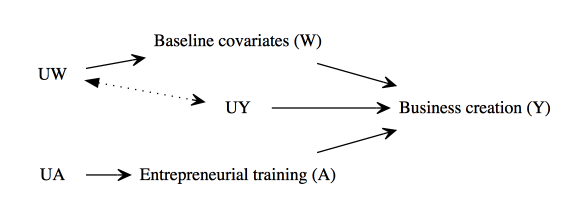
\includegraphics{../../DAG_Uganda.png}
  \caption{Figure 1: Structural causal model\label{fig:DAG}}
\end{figure}



\section{Variables of interest}
\label{sec:variables-interest}


\begin{center}
\begin{tabular}{ | p{0.15\linewidth} | p{0.3\linewidth} |  p{0.45\linewidth} | } 
 \hline
 Variable type & Variable name & Description \\ 

\hline
 $Y$ & Business creation & =1 if respondent started a business after graduation from high school \\ 

\hline
 $Y$ &Log of revenue & Monthly revenue from all self-employment activities \\ 

\hline 
$Y$ & Log of profit & Monthly profit from all self-employment activities \\

\hline
$A$ & Treatment & =1 if participated in entrepreneurial training \\

\hline
$W$ & Sociodemographic characteristics & Gender, age, parent’s income source and education level, boarding student, perceived socioeconomic level \\

\hline
$W$ & Cognitive skills & Raven score, math score, GPA, O-level score, previous exposure to entrepreneurship  \\

\hline
$W$ & Risk and time preferences & Present-bias and time-inconsistency scores \\

\hline
$W$ & Personality characteristics & Big 5 (extroversion, emotional stability, openness, conscientiousness, agreeableness), leadership, perceived control, anxiety, pro-social behavior, and more. \\

 \hline
\end{tabular}
\end{center}

%%% Local Variables:
%%% mode: latex
%%% TeX-master: "main/report"
%%% End:


\section{Interpretation}
\label{sec:interpretation}

\section{Future Directions}
\label{sec:future-directions}

In future work we would like to investigate the differences in effectiveness, if any, between the hard-skills and soft-skills training. For the purposes of this initial analysis, we pooled both treatment pools into a single group. However, understanding the differences between the two treatment modes would have real policy implications: most existing entrepreneurship training programs only employ hard-skills training. Governments interested in effectively training their entrepreneurs would like to know whether hard-skills training, soft-skills training, or a combination of both, is most likely to improve the economic outcomes of the trainees. This was a question we completely neglected in the present analysis.

\printbibliography


\chapter{Appendices}
\label{cha:appendices}



\section{Code for Analysis}
\label{sec:appendix-1}


  \begin{Verbatim}[commandchars=\\\{\}]
{\color{incolor}In [{\color{incolor}1}]:} \PY{c+c1}{\PYZsh{} Note: for full reproducibility of results, we should have set the random seed earlier.}
        \PY{k+kp}{set.seed}\PY{p}{(}\PY{l+m}{518}\PY{p}{)}
        \PY{c+c1}{\PYZsh{} The values generated are similar to those from the slides, but not the same.}
        
        \PY{k+kp}{rm}\PY{p}{(}\PY{k+kt}{list}\PY{o}{=}\PY{k+kp}{ls}\PY{p}{(}\PY{p}{)}\PY{p}{)}
        \PY{c+c1}{\PYZsh{} William: commented out below for notebook}
        \PY{c+c1}{\PYZsh{} knitr::opts\PYZus{}chunk\PYZdl{}set(echo = TRUE)}
        \PY{k+kp}{getwd}\PY{p}{(}\PY{p}{)}
        \PY{k+kp}{options}\PY{p}{(}scipen\PY{o}{=}\PY{l+m}{10}\PY{p}{)}
        
        \PY{c+c1}{\PYZsh{} William: prevent excessive verbosity}
        \PY{k+kp}{suppressMessages}\PY{p}{(}   \PY{k+kn}{library}\PY{p}{(}tmle\PY{p}{)}\PY{p}{)}
        \PY{c+c1}{\PYZsh{} William: prevent excessive verbosity}
        \PY{k+kp}{suppressMessages}\PY{p}{(}   \PY{k+kn}{library}\PY{p}{(}ggplot2\PY{p}{)}\PY{p}{)}
                            \PY{k+kn}{library}\PY{p}{(}SuperLearner\PY{p}{)}
        \PY{c+c1}{\PYZsh{} William: prevent excessive verbosity}
        \PY{k+kp}{suppressMessages}\PY{p}{(}   \PY{k+kn}{library}\PY{p}{(}dplyr\PY{p}{)}\PY{p}{)}
                            \PY{k+kn}{library}\PY{p}{(}magrittr\PY{p}{)}
        \PY{c+c1}{\PYZsh{} William: commented this out because obviously isn\PYZsq{}t necessary for notebook}
        \PY{c+c1}{\PYZsh{}                   library(knitr)}
                            \PY{k+kn}{library}\PY{p}{(}foreign\PY{p}{)}
                            \PY{k+kn}{library}\PY{p}{(}ck37r\PY{p}{)}
        \PY{k+kp}{suppressMessages}\PY{p}{(}   \PY{k+kn}{library}\PY{p}{(}sl3\PY{p}{)}\PY{p}{)}
        \PY{k+kp}{suppressMessages}\PY{p}{(}   \PY{k+kn}{library}\PY{p}{(}arm\PY{p}{)}\PY{p}{)}
        \PY{c+c1}{\PYZsh{} William: added this line to prevent verbosity from caret}
                            \PY{k+kn}{library}\PY{p}{(}lattice\PY{p}{)}
                            \PY{k+kn}{library}\PY{p}{(}caret\PY{p}{)}
        \PY{k+kp}{suppressMessages}\PY{p}{(}   \PY{k+kn}{library}\PY{p}{(}data.table\PY{p}{)}\PY{p}{)}
                            \PY{k+kn}{library}\PY{p}{(}screening\PY{p}{)}
        \PY{c+c1}{\PYZsh{} William: added this line so that SuperLearner calls will work}
        \PY{k+kp}{suppressMessages}\PY{p}{(}   \PY{k+kn}{library}\PY{p}{(}xgboost\PY{p}{)}\PY{p}{)}
        \PY{c+c1}{\PYZsh{} William: added these two lines to prevent unnecessary warnings when screening() is called}
                            \PY{k+kn}{library}\PY{p}{(}foreach\PY{p}{)}
        \PY{k+kp}{suppressMessages}\PY{p}{(}   \PY{k+kn}{library}\PY{p}{(}glmnet\PY{p}{)}\PY{p}{)}
\end{Verbatim}

%%% Local Variables:
%%% mode: latex
%%% TeX-master: "../main/report"
%%% End:


   \begin{Verbatim}[commandchars=\\\{\}]
{\color{incolor}In [{\color{incolor}2}]:} data \PY{o}{\PYZlt{}\PYZhy{}} read.dta\PY{p}{(}\PY{l+s}{\PYZdq{}}\PY{l+s}{Data/SEED\PYZus{}endline\PYZus{}analysis.dta\PYZdq{}}\PY{p}{,}
                     convert.factors\PY{o}{=}\PY{k+kc}{FALSE}\PY{p}{,} convert.underscore\PY{o}{=}\PY{k+kc}{FALSE}\PY{p}{)}
        data \PY{o}{\PYZlt{}\PYZhy{}} \PY{k+kt}{data.frame}\PY{p}{(}data\PY{p}{)}
\end{Verbatim}

%%% Local Variables:
%%% mode: latex
%%% TeX-master: "../main/report"
%%% End:


   \begin{Verbatim}[commandchars=\\\{\}]
{\color{incolor}In [{\color{incolor}3}]:} \PY{c+c1}{\PYZsh{} List to hold the different column names.}
        \PY{p}{(}names\PY{o}{=}\PY{k+kt}{list}\PY{p}{(}
          \PY{c+c1}{\PYZsh{} Outcomes of interest}
          outcome\PY{o}{=}\PY{k+kt}{c}\PY{p}{(}\PY{l+s}{\PYZdq{}}\PY{l+s}{ever\PYZus{}self\PYZus{}employed\PYZdq{}}\PY{p}{,}\PY{l+s}{\PYZdq{}}\PY{l+s}{log\PYZus{}tot\PYZdq{}}\PY{p}{)}\PY{p}{,}
        
          \PY{c+c1}{\PYZsh{} Treatment variable}
          treatment\PY{o}{=}\PY{l+s}{\PYZdq{}}\PY{l+s}{treated\PYZdq{}}\PY{p}{,}
        
          \PY{c+c1}{\PYZsh{} Adjustment covariates}
          covars\PY{o}{=}\PY{k+kt}{c}\PY{p}{(}\PY{l+s}{\PYZdq{}}\PY{l+s}{treated\PYZdq{}}\PY{p}{,}\PY{l+s}{\PYZdq{}}\PY{l+s}{gender\PYZdq{}}\PY{p}{,}\PY{l+s}{\PYZdq{}}\PY{l+s}{age\PYZdq{}}\PY{p}{,}\PY{l+s}{\PYZdq{}}\PY{l+s}{q06\PYZus{}dayorboarding\PYZdq{}}\PY{p}{,}
          \PY{l+s}{\PYZdq{}}\PY{l+s}{q25\PYZus{}family\PYZus{}business\PYZdq{}}\PY{p}{,}\PY{l+s}{\PYZdq{}}\PY{l+s}{q25a\PYZus{}wk\PYZus{}family\PYZus{}bus\PYZdq{}}\PY{p}{,}\PY{l+s}{\PYZdq{}}\PY{l+s}{timeprefs\PYZus{}patience\PYZdq{}}\PY{p}{,}
          \PY{l+s}{\PYZdq{}}\PY{l+s}{riskbehavior\PYZdq{}}\PY{p}{,}\PY{l+s}{\PYZdq{}}\PY{l+s}{mathbusiness\PYZdq{}}\PY{p}{,}\PY{l+s}{\PYZdq{}}\PY{l+s}{leadership\PYZdq{}}\PY{p}{,}\PY{l+s}{\PYZdq{}}\PY{l+s}{perceivedcontrol\PYZdq{}}\PY{p}{,}\PY{l+s}{\PYZdq{}}\PY{l+s}{timeprefs\PYZus{}delta\PYZdq{}}\PY{p}{,}
          \PY{l+s}{\PYZdq{}}\PY{l+s}{timeprefs\PYZus{}beta\PYZdq{}}\PY{p}{,}\PY{l+s}{\PYZdq{}}\PY{l+s}{prosocialbehavior\PYZdq{}}\PY{p}{,}\PY{l+s}{\PYZdq{}}\PY{l+s}{anxiety\PYZdq{}}\PY{p}{,}\PY{l+s}{\PYZdq{}}\PY{l+s}{selfconfidence\PYZdq{}}\PY{p}{,}
          \PY{l+s}{\PYZdq{}}\PY{l+s}{big5extroversion\PYZdq{}}\PY{p}{,}\PY{l+s}{\PYZdq{}}\PY{l+s}{big5emostability\PYZdq{}}\PY{p}{,}\PY{l+s}{\PYZdq{}}\PY{l+s}{big5openness\PYZdq{}}\PY{p}{,}\PY{l+s}{\PYZdq{}}\PY{l+s}{big5conscientious\PYZdq{}}\PY{p}{,}
          \PY{l+s}{\PYZdq{}}\PY{l+s}{big5agreeable\PYZdq{}}\PY{p}{,}\PY{l+s}{\PYZdq{}}\PY{l+s}{schoolacceptance\PYZdq{}}\PY{p}{,}\PY{l+s}{\PYZdq{}}\PY{l+s}{currfamwealthstep\PYZdq{}}\PY{p}{,}\PY{l+s}{\PYZdq{}}\PY{l+s}{tenyrwealthstep\PYZdq{}}\PY{p}{,}\PY{l+s}{\PYZdq{}}\PY{l+s}{takingriskstep\PYZdq{}}\PY{p}{,}
          \PY{l+s}{\PYZdq{}}\PY{l+s}{ravenscore\PYZdq{}}\PY{p}{,}\PY{l+s}{\PYZdq{}}\PY{l+s}{father\PYZus{}educ2\PYZdq{}}\PY{p}{,}\PY{l+s}{\PYZdq{}}\PY{l+s}{father\PYZus{}educ3\PYZdq{}}\PY{p}{,}\PY{l+s}{\PYZdq{}}\PY{l+s}{father\PYZus{}educ4\PYZdq{}}\PY{p}{,}\PY{l+s}{\PYZdq{}}\PY{l+s}{father\PYZus{}educ5\PYZdq{}}\PY{p}{,}
          \PY{l+s}{\PYZdq{}}\PY{l+s}{father\PYZus{}income2\PYZdq{}}\PY{p}{,}\PY{l+s}{\PYZdq{}}\PY{l+s}{father\PYZus{}income3\PYZdq{}}\PY{p}{,}\PY{l+s}{\PYZdq{}}\PY{l+s}{mother\PYZus{}income2\PYZdq{}}\PY{p}{,}\PY{l+s}{\PYZdq{}}\PY{l+s}{mother\PYZus{}income3\PYZdq{}}\PY{p}{,}
          \PY{l+s}{\PYZdq{}}\PY{l+s}{type\PYZus{}house\PYZdq{}}\PY{p}{,}\PY{l+s}{\PYZdq{}}\PY{l+s}{q13\PYZus{}olevelscore2\PYZdq{}}\PY{p}{,}\PY{l+s}{\PYZdq{}}\PY{l+s}{q13\PYZus{}olevelscore34\PYZdq{}}\PY{p}{)}
        \PY{p}{)}\PY{p}{)}
\end{Verbatim}


\textbf{\$outcome} \\
 \mbox{'ever\_self\_employed'} \hspace{6pt} \mbox{'log\_tot'}\\


\textbf{\$treatment}\\ 
\mbox{'treated'}
\\

\textbf{\$covars} \\
 \mbox{'treated'} \hspace{6pt}
 \mbox{'gender'} \hspace{6pt}
 \mbox{'age'} \hspace{6pt}
 \mbox{'q06\_dayorboarding'} \hspace{6pt}
 \mbox{'q25\_family\_business'} \hspace{6pt}
 \mbox{'q25a\_wk\_family\_bus'} \hspace{6pt}
 \mbox{'timeprefs\_patience'} \hspace{6pt}
 \mbox{'riskbehavior'} \hspace{6pt}
 \mbox{'mathbusiness'} \hspace{6pt}
 \mbox{'leadership'} \hspace{6pt}
 \mbox{'perceivedcontrol'} \hspace{6pt}
 \mbox{'timeprefs\_delta'} \hspace{6pt}
 \mbox{'timeprefs\_beta'} \hspace{6pt}
 \mbox{'prosocialbehavior'} \hspace{6pt}
 \mbox{'anxiety'} \hspace{6pt}
 \mbox{'selfconfidence'} \hspace{6pt}
 \mbox{'big5extroversion'} \hspace{6pt}
 \mbox{'big5emostability'} \hspace{6pt}
 \mbox{'big5openness'} \hspace{6pt}
 \mbox{'big5conscientious'} \hspace{6pt}
 \mbox{'big5agreeable'} \hspace{6pt}
 \mbox{'schoolacceptance'} \hspace{6pt}
 \mbox{'currfamwealthstep'} \hspace{6pt}
 \mbox{'tenyrwealthstep'} \hspace{6pt}
 \mbox{'takingriskstep'} \hspace{6pt}
 \mbox{'ravenscore'} \hspace{6pt}
 \mbox{'father\_educ2'} \hspace{6pt}
 \mbox{'father\_educ3'} \hspace{6pt}
 \mbox{'father\_educ4'} \hspace{6pt}
 \mbox{'father\_educ5'} \hspace{6pt}
 \mbox{'father\_income2'} \hspace{6pt}
 \mbox{'father\_income3'} \hspace{6pt}
 \mbox{'mother\_income2'} \hspace{6pt}
 \mbox{'mother\_income3'} \hspace{6pt}
 \mbox{'type\_house'} \hspace{6pt}
 \mbox{'q13\_olevelscore2'} \hspace{6pt}
 \mbox{'q13\_olevelscore34'}



%%% Local Variables:
%%% mode: latex
%%% TeX-master: "../main/report"
%%% End:


   \begin{Verbatim}[commandchars=\\\{\}]
{\color{incolor}In [{\color{incolor}4}]:} \PY{c+c1}{\PYZsh{} Keep variables of interest}
        
        data \PY{o}{\PYZlt{}\PYZhy{}} \PY{k+kp}{subset}\PY{p}{(}data\PY{p}{,} select\PY{o}{=}\PY{k+kt}{c}\PY{p}{(}\PY{k+kp}{names}\PY{o}{\PYZdl{}}outcome\PY{p}{,} \PY{k+kp}{names}\PY{o}{\PYZdl{}}treatment\PY{p}{,} \PY{k+kp}{names}\PY{o}{\PYZdl{}}covars\PY{p}{)}\PY{p}{)}
        \PY{c+c1}{\PYZsh{} Review missing values in id, outcome, treatment, and censoring variables.}
        \PY{c+c1}{\PYZsh{} Outcome is the only variable that can have missing values.}
        \PY{k+kp}{colSums}\PY{p}{(}\PY{k+kp}{is.na}\PY{p}{(}data\PY{p}{[}\PY{p}{,} \PY{k+kt}{c}\PY{p}{(}\PY{k+kp}{names}\PY{o}{\PYZdl{}}outcome\PY{p}{,} \PY{k+kp}{names}\PY{o}{\PYZdl{}}censoring\PY{p}{,} \PY{k+kp}{names}\PY{o}{\PYZdl{}}treatment\PY{p}{)}\PY{p}{]}\PY{p}{)}\PY{p}{)}
\end{Verbatim}


    \begin{description*}
\item[ever\textbackslash{}\_self\textbackslash{}\_employed] 0
\item[log\textbackslash{}\_tot] 712
\item[treated] 0
\end{description*}


 

   \begin{Verbatim}[commandchars=\\\{\}]
{\color{incolor}In [{\color{incolor}5}]:} \PY{c+c1}{\PYZsh{} Dimensions of data set}
        \PY{k+kp}{dim}\PY{p}{(}data\PY{p}{)}
\end{Verbatim}


    \begin{enumerate*}
\item 3891
\item 40
\end{enumerate*}


   \begin{Verbatim}[commandchars=\\\{\}]
{\color{incolor}In [{\color{incolor}6}]:} \PY{c+c1}{\PYZsh{} Summary statistics of data set}
        \PY{k+kp}{summary}\PY{p}{(}data\PY{p}{)}
\end{Verbatim}


    
    \begin{verbatim}
 ever_self_employed    log_tot          treated         treated.1     
 Min.   :0.0000     Min.   : 1.028   Min.   :0.0000   Min.   :0.0000  
 1st Qu.:0.0000     1st Qu.: 6.580   1st Qu.:0.0000   1st Qu.:0.0000  
 Median :1.0000     Median : 7.681   Median :1.0000   Median :1.0000  
 Mean   :0.5474     Mean   : 7.593   Mean   :0.7376   Mean   :0.7376  
 3rd Qu.:1.0000     3rd Qu.: 8.645   3rd Qu.:1.0000   3rd Qu.:1.0000  
 Max.   :1.0000     Max.   :11.018   Max.   :1.0000   Max.   :1.0000  
                    NA's   :712                                       
     gender            age        q06_dayorboarding q25_family_business
 Min.   :0.0000   Min.   :20.00   Min.   :0.0000    Min.   :0.0000     
 1st Qu.:0.0000   1st Qu.:22.00   1st Qu.:0.0000    1st Qu.:0.0000     
 Median :0.0000   Median :23.00   Median :1.0000    Median :1.0000     
 Mean   :0.3482   Mean   :23.51   Mean   :0.7396    Mean   :0.5193     
 3rd Qu.:1.0000   3rd Qu.:24.00   3rd Qu.:1.0000    3rd Qu.:1.0000     
 Max.   :1.0000   Max.   :38.00   Max.   :1.0000    Max.   :1.0000     
                                  NA's   :147       NA's   :13         
 q25a_wk_family_bus timeprefs_patience  riskbehavior        mathbusiness   
 Min.   :0.0000     Min.   :0.0000     Min.   :-2.538293   Min.   :0.0000  
 1st Qu.:1.0000     1st Qu.:0.0000     1st Qu.:-0.692131   1st Qu.:0.5000  
 Median :1.0000     Median :0.0000     Median :-0.083936   Median :0.6667  
 Mean   :0.9276     Mean   :0.2765     Mean   :-0.002497   Mean   :0.5990  
 3rd Qu.:1.0000     3rd Qu.:0.3333     3rd Qu.: 0.656105   3rd Qu.:0.7500  
 Max.   :1.0000     Max.   :1.0000     Max.   : 2.965215   Max.   :1.0000  
 NA's   :1860                                                              
   leadership    perceivedcontrol timeprefs_delta     timeprefs_beta     
 Min.   :1.000   Min.   :1.000    Min.   :-3.299497   Min.   :-3.048114  
 1st Qu.:3.857   1st Qu.:4.167    1st Qu.:-0.662538   1st Qu.:-0.682101  
 Median :4.286   Median :4.333    Median : 0.001506   Median :-0.013883  
 Mean   :4.194   Mean   :4.337    Mean   : 0.001506   Mean   : 0.002516  
 3rd Qu.:4.571   3rd Qu.:4.667    3rd Qu.: 0.643275   3rd Qu.: 0.637755  
 Max.   :5.000   Max.   :5.000    Max.   : 3.363326   Max.   : 3.857732  
 NA's   :23      NA's   :14                                              
 prosocialbehavior    anxiety      selfconfidence  big5extroversion
 Min.   :1.000     Min.   :1.000   Min.   :1.000   Min.   :1.000   
 1st Qu.:4.000     1st Qu.:1.889   1st Qu.:4.333   1st Qu.:2.000   
 Median :4.293     Median :2.333   Median :4.667   Median :3.000   
 Mean   :4.293     Mean   :2.391   Mean   :4.583   Mean   :2.733   
 3rd Qu.:4.714     3rd Qu.:2.875   3rd Qu.:5.000   3rd Qu.:3.500   
 Max.   :5.000     Max.   :5.000   Max.   :5.000   Max.   :5.000   
                   NA's   :28      NA's   :37                      
 big5emostability  big5openness   big5conscientious big5agreeable 
 Min.   :1.000    Min.   :1.000   Min.   :1.000     Min.   :1.00  
 1st Qu.:3.500    1st Qu.:3.500   1st Qu.:3.500     1st Qu.:3.00  
 Median :4.000    Median :4.151   Median :4.000     Median :3.50  
 Mean   :3.865    Mean   :4.151   Mean   :3.892     Mean   :3.62  
 3rd Qu.:4.500    3rd Qu.:5.000   3rd Qu.:4.500     3rd Qu.:4.00  
 Max.   :5.000    Max.   :5.000   Max.   :5.000     Max.   :5.00  
                                                                  
 schoolacceptance currfamwealthstep tenyrwealthstep  takingriskstep  
 Min.   :1.000    Min.   : 1.000    Min.   : 1.000   Min.   : 1.000  
 1st Qu.:4.000    1st Qu.: 4.000    1st Qu.: 7.000   1st Qu.: 5.000  
 Median :4.250    Median : 5.000    Median : 8.000   Median : 7.000  
 Mean   :4.268    Mean   : 4.776    Mean   : 8.015   Mean   : 6.756  
 3rd Qu.:4.750    3rd Qu.: 6.000    3rd Qu.: 9.000   3rd Qu.: 9.000  
 Max.   :5.000    Max.   :10.000    Max.   :10.000   Max.   :10.000  
 NA's   :91       NA's   :83        NA's   :81       NA's   :88      
   ravenscore      father_educ2     father_educ3   father_educ4   
 Min.   : 0.000   Min.   :0.0000   Min.   :0.00   Min.   :0.0000  
 1st Qu.: 4.000   1st Qu.:0.0000   1st Qu.:0.00   1st Qu.:0.0000  
 Median : 6.000   Median :0.0000   Median :0.00   Median :0.0000  
 Mean   : 5.435   Mean   :0.1667   Mean   :0.13   Mean   :0.1838  
 3rd Qu.: 7.000   3rd Qu.:0.0000   3rd Qu.:0.00   3rd Qu.:0.0000  
 Max.   :10.000   Max.   :1.0000   Max.   :1.00   Max.   :1.0000  
                  NA's   :28       NA's   :28     NA's   :28      
  father_educ5    father_income2   father_income3   mother_income2  
 Min.   :0.0000   Min.   :0.0000   Min.   :0.0000   Min.   :0.0000  
 1st Qu.:0.0000   1st Qu.:0.0000   1st Qu.:0.0000   1st Qu.:0.0000  
 Median :0.0000   Median :0.0000   Median :0.0000   Median :0.0000  
 Mean   :0.4072   Mean   :0.2924   Mean   :0.0384   Mean   :0.1553  
 3rd Qu.:1.0000   3rd Qu.:1.0000   3rd Qu.:0.0000   3rd Qu.:0.0000  
 Max.   :1.0000   Max.   :1.0000   Max.   :1.0000   Max.   :1.0000  
 NA's   :28       NA's   :37       NA's   :37       NA's   :15      
 mother_income3      type_house     q13_olevelscore2 q13_olevelscore34
 Min.   :0.00000   Min.   :0.0000   Min.   :0.0000   Min.   :0.0000   
 1st Qu.:0.00000   1st Qu.:1.0000   1st Qu.:0.0000   1st Qu.:0.0000   
 Median :0.00000   Median :1.0000   Median :0.0000   Median :0.0000   
 Mean   :0.03199   Mean   :0.8205   Mean   :0.4014   Mean   :0.4522   
 3rd Qu.:0.00000   3rd Qu.:1.0000   3rd Qu.:1.0000   3rd Qu.:1.0000   
 Max.   :1.00000   Max.   :1.0000   Max.   :1.0000   Max.   :1.0000   
 NA's   :15        NA's   :24       NA's   :72       NA's   :72       
    \end{verbatim}

 

   \begin{Verbatim}[commandchars=\\\{\}]
{\color{incolor}In [{\color{incolor}7}]:} \PY{c+c1}{\PYZsh{} Remove observations missing their censoring time.}
        skip\PYZus{}vars \PY{o}{\PYZlt{}\PYZhy{}} \PY{k+kt}{c}\PY{p}{(}\PY{k+kp}{names}\PY{o}{\PYZdl{}}treatment\PY{p}{,} \PY{k+kp}{names}\PY{o}{\PYZdl{}}outcome\PY{p}{)}
        impute \PY{o}{\PYZlt{}\PYZhy{}} ck37r\PY{o}{::}impute\PYZus{}missing\PYZus{}values\PY{p}{(}data\PY{p}{,}
                                               skip\PYZus{}vars\PY{o}{=}skip\PYZus{}vars\PY{p}{)}
\end{Verbatim}

%%% Local Variables:
%%% mode: latex
%%% TeX-master: "../main/report"
%%% End:


  \begin{Verbatim}[commandchars=\\\{\}]
{\color{incolor}In [{\color{incolor}8}]:} \PY{c+c1}{\PYZsh{} Review missing data for all covariates.}
        \PY{c+c1}{\PYZsh{} Only the outcome variable should have missing data at this point.}
        data \PY{o}{\PYZlt{}\PYZhy{}} impute\PY{o}{\PYZdl{}}data
        
        \PY{k+kp}{colSums}\PY{p}{(}\PY{k+kp}{is.na}\PY{p}{(}data\PY{p}{)}\PY{p}{)}
\end{Verbatim}


    \begin{description*}
\item[ever\textbackslash{}\_self\textbackslash{}\_employed] 0
\item[log\textbackslash{}\_tot] 712
\item[treated] 0
\item[treated.1] 0
\item[gender] 0
\item[age] 0
\item[q06\textbackslash{}\_dayorboarding] 0
\item[q25\textbackslash{}\_family\textbackslash{}\_business] 0
\item[q25a\textbackslash{}\_wk\textbackslash{}\_family\textbackslash{}\_bus] 0
\item[timeprefs\textbackslash{}\_patience] 0
\item[riskbehavior] 0
\item[mathbusiness] 0
\item[leadership] 0
\item[perceivedcontrol] 0
\item[timeprefs\textbackslash{}\_delta] 0
\item[timeprefs\textbackslash{}\_beta] 0
\item[prosocialbehavior] 0
\item[anxiety] 0
\item[selfconfidence] 0
\item[big5extroversion] 0
\item[big5emostability] 0
\item[big5openness] 0
\item[big5conscientious] 0
\item[big5agreeable] 0
\item[schoolacceptance] 0
\item[currfamwealthstep] 0
\item[tenyrwealthstep] 0
\item[takingriskstep] 0
\item[ravenscore] 0
\item[father\textbackslash{}\_educ2] 0
\item[father\textbackslash{}\_educ3] 0
\item[father\textbackslash{}\_educ4] 0
\item[father\textbackslash{}\_educ5] 0
\item[father\textbackslash{}\_income2] 0
\item[father\textbackslash{}\_income3] 0
\item[mother\textbackslash{}\_income2] 0
\item[mother\textbackslash{}\_income3] 0
\item[type\textbackslash{}\_house] 0
\item[q13\textbackslash{}\_olevelscore2] 0
\item[q13\textbackslash{}\_olevelscore34] 0
\item[miss\textbackslash{}\_log\textbackslash{}\_tot] 0
\item[miss\textbackslash{}\_q06\textbackslash{}\_dayorboarding] 0
\item[miss\textbackslash{}\_q25\textbackslash{}\_family\textbackslash{}\_business] 0
\item[miss\textbackslash{}\_q25a\textbackslash{}\_wk\textbackslash{}\_family\textbackslash{}\_bus] 0
\item[miss\textbackslash{}\_leadership] 0
\item[miss\textbackslash{}\_perceivedcontrol] 0
\item[miss\textbackslash{}\_anxiety] 0
\item[miss\textbackslash{}\_selfconfidence] 0
\item[miss\textbackslash{}\_schoolacceptance] 0
\item[miss\textbackslash{}\_currfamwealthstep] 0
\item[miss\textbackslash{}\_tenyrwealthstep] 0
\item[miss\textbackslash{}\_takingriskstep] 0
\item[miss\textbackslash{}\_father\textbackslash{}\_educ2] 0
\item[miss\textbackslash{}\_father\textbackslash{}\_income2] 0
\item[miss\textbackslash{}\_mother\textbackslash{}\_income2] 0
\item[miss\textbackslash{}\_type\textbackslash{}\_house] 0
\item[miss\textbackslash{}\_q13\textbackslash{}\_olevelscore2] 0
\end{description*}


  
%%% Local Variables:
%%% mode: latex
%%% TeX-master: "../main/report"
%%% End:


  \begin{Verbatim}[commandchars=\\\{\}]
{\color{incolor}In [{\color{incolor}9}]:} \PY{c+c1}{\PYZsh{}\PYZsh{} Estimation of causal efects}
        
        Y1 \PY{o}{\PYZlt{}\PYZhy{}} data\PY{o}{\PYZdl{}}ever\PYZus{}self\PYZus{}employed
        Y2 \PY{o}{\PYZlt{}\PYZhy{}} data\PY{o}{\PYZdl{}}log\PYZus{}tot\PY{p}{[}\PY{o}{!}\PY{k+kp}{is.na}\PY{p}{(}data\PY{o}{\PYZdl{}}log\PYZus{}tot\PY{p}{)}\PY{p}{]}
        
        A1 \PY{o}{\PYZlt{}\PYZhy{}} data\PY{o}{\PYZdl{}}treated
        A2 \PY{o}{\PYZlt{}\PYZhy{}} data\PY{o}{\PYZdl{}}treated\PY{p}{[}\PY{o}{!}\PY{k+kp}{is.na}\PY{p}{(}data\PY{o}{\PYZdl{}}log\PYZus{}tot\PY{p}{)}\PY{p}{]}
        
        all\PYZus{}covars \PY{o}{\PYZlt{}\PYZhy{}} data\PY{p}{[}\PY{p}{,} \PY{k+kp}{colnames}\PY{p}{(}data\PY{p}{)} \PY{o}{\PYZpc{}in\PYZpc{}} \PY{k+kp}{names}\PY{o}{\PYZdl{}}covars\PY{p}{]}
        
        W \PY{o}{\PYZlt{}\PYZhy{}}  all\PYZus{}covars
        W1 \PY{o}{\PYZlt{}\PYZhy{}} all\PYZus{}covars
        W2 \PY{o}{\PYZlt{}\PYZhy{}} \PY{k+kp}{subset}\PY{p}{(}data\PY{p}{,} \PY{o}{!}\PY{k+kp}{is.na}\PY{p}{(}data\PY{o}{\PYZdl{}}log\PYZus{}tot\PY{p}{)}\PY{p}{)}
        W2 \PY{o}{\PYZlt{}\PYZhy{}} W2\PY{p}{[}\PY{p}{,} \PY{k+kp}{colnames}\PY{p}{(}data\PY{p}{)} \PY{o}{\PYZpc{}in\PYZpc{}} \PY{k+kp}{names}\PY{o}{\PYZdl{}}covars\PY{p}{]}
        
        screen1 \PY{o}{\PYZlt{}\PYZhy{}}  screening\PY{p}{(}x\PY{o}{=}W1\PY{p}{,} y\PY{o}{=}Y1\PY{p}{,} method\PY{o}{=}\PY{l+s}{\PYZdq{}}\PY{l+s}{holp\PYZdq{}}\PY{p}{,} family\PY{o}{=}\PY{l+s}{\PYZdq{}}\PY{l+s}{binomial\PYZdq{}}\PY{p}{,} num.select\PY{o}{=}\PY{l+m}{15}\PY{p}{)}\PY{o}{\PYZdl{}}screen
        screen2 \PY{o}{\PYZlt{}\PYZhy{}}  screening\PY{p}{(}x\PY{o}{=}W2\PY{p}{,} y\PY{o}{=}Y2\PY{p}{,} method\PY{o}{=}\PY{l+s}{\PYZdq{}}\PY{l+s}{holp\PYZdq{}}\PY{p}{,} family\PY{o}{=}\PY{l+s}{\PYZdq{}}\PY{l+s}{gaussian\PYZdq{}}\PY{p}{,} num.select\PY{o}{=}\PY{l+m}{15}\PY{p}{)}\PY{o}{\PYZdl{}}screen
        screenA \PY{o}{\PYZlt{}\PYZhy{}}  screening\PY{p}{(}x\PY{o}{=}W\PY{p}{,}  y\PY{o}{=}A1\PY{p}{,} method\PY{o}{=}\PY{l+s}{\PYZdq{}}\PY{l+s}{holp\PYZdq{}}\PY{p}{,} family\PY{o}{=}\PY{l+s}{\PYZdq{}}\PY{l+s}{binomial\PYZdq{}}\PY{p}{,} num.select\PY{o}{=}\PY{l+m}{15}\PY{p}{)}\PY{o}{\PYZdl{}}screen 
        screenA2 \PY{o}{\PYZlt{}\PYZhy{}} screening\PY{p}{(}x\PY{o}{=}W2\PY{p}{,} y\PY{o}{=}A2\PY{p}{,} method\PY{o}{=}\PY{l+s}{\PYZdq{}}\PY{l+s}{holp\PYZdq{}}\PY{p}{,} family\PY{o}{=}\PY{l+s}{\PYZdq{}}\PY{l+s}{binomial\PYZdq{}}\PY{p}{,} num.select\PY{o}{=}\PY{l+m}{15}\PY{p}{)}\PY{o}{\PYZdl{}}screen 
        
        W1 \PY{o}{\PYZlt{}\PYZhy{}} W1\PY{p}{[}\PY{p}{,}screen1\PY{p}{]}
        W2 \PY{o}{\PYZlt{}\PYZhy{}} W2\PY{p}{[}\PY{p}{,}screen2\PY{p}{]}
        
        \PY{c+c1}{\PYZsh{} William: added/moved this line here to make code work}
        screenA2 \PY{o}{\PYZlt{}\PYZhy{}} screening\PY{p}{(}x\PY{o}{=}W2\PY{p}{,} y\PY{o}{=}A2\PY{p}{,} method\PY{o}{=}\PY{l+s}{\PYZdq{}}\PY{l+s}{holp\PYZdq{}}\PY{p}{,} family\PY{o}{=}\PY{l+s}{\PYZdq{}}\PY{l+s}{binomial\PYZdq{}}\PY{p}{,} num.select\PY{o}{=}\PY{l+m}{15}\PY{p}{)}\PY{o}{\PYZdl{}}screen 
        \PY{c+c1}{\PYZsh{} screenA2 depends on W2, and W2 was changed above, so old screenA2 couldn\PYZsq{}t be used to subset new W2}
        
        WA \PY{o}{\PYZlt{}\PYZhy{}}  W\PY{p}{[} \PY{p}{,}screenA\PY{p}{]}
        WA2 \PY{o}{\PYZlt{}\PYZhy{}} W2\PY{p}{[}\PY{p}{,}screenA2\PY{p}{]}
\end{Verbatim}



 \begin{Verbatim}[commandchars=\\\{\}]
{\color{incolor}In [{\color{incolor}10}]:} \PY{c+c1}{\PYZsh{} Fit glm model (base model, should have the worst performance)}
         
         logit2prob \PY{o}{\PYZlt{}\PYZhy{}} \PY{k+kr}{function}\PY{p}{(}logit\PY{p}{)}\PY{p}{\PYZob{}}
           odds \PY{o}{\PYZlt{}\PYZhy{}} \PY{k+kp}{exp}\PY{p}{(}logit\PY{p}{)}
           prob \PY{o}{\PYZlt{}\PYZhy{}} odds \PY{o}{/} \PY{p}{(}\PY{l+m}{1} \PY{o}{+} odds\PY{p}{)}
           \PY{k+kr}{return}\PY{p}{(}prob\PY{p}{)}
         \PY{p}{\PYZcb{}}
         
         model1 \PY{o}{\PYZlt{}\PYZhy{}} glm\PY{p}{(}formula\PY{o}{=}Y1 \PY{o}{\PYZti{}} A1\PY{p}{,} family\PY{o}{=}\PY{l+s}{\PYZdq{}}\PY{l+s}{binomial\PYZdq{}}\PY{p}{)}
         \PY{k+kp}{summary}\PY{p}{(}model1\PY{p}{)}
\end{Verbatim}


    
    \begin{verbatim}

Call:
glm(formula = Y1 ~ A1, family = "binomial")

Deviance Residuals: 
   Min      1Q  Median      3Q     Max  
-1.306  -1.306   1.054   1.054   1.224  

Coefficients:
            Estimate Std. Error z value   Pr(>|z|)    
(Intercept) -0.10784    0.06268  -1.720     0.0854 .  
A1           0.40549    0.07317   5.542 0.00000003 ***
---
Signif. codes:  0 ‘***’ 0.001 ‘**’ 0.01 ‘*’ 0.05 ‘.’ 0.1 ‘ ’ 1

(Dispersion parameter for binomial family taken to be 1)

    Null deviance: 5359.0  on 3890  degrees of freedom
Residual deviance: 5328.2  on 3889  degrees of freedom
AIC: 5332.2

Number of Fisher Scoring iterations: 4

    \end{verbatim}

   
%%% Local Variables:
%%% mode: latex
%%% TeX-master: "../main/report"
%%% End:



    \begin{Verbatim}[commandchars=\\\{\}]
{\color{incolor}In [{\color{incolor}11}]:} logit\PYZus{}control \PY{o}{\PYZlt{}\PYZhy{}} model1\PY{o}{\PYZdl{}}coefficients\PY{p}{[}\PY{l+m}{1}\PY{p}{]}
         logit\PYZus{}treated \PY{o}{\PYZlt{}\PYZhy{}} model1\PY{o}{\PYZdl{}}coefficients\PY{p}{[}\PY{l+m}{1}\PY{p}{]} \PY{o}{+} \PY{l+m}{1}\PY{o}{*}model1\PY{o}{\PYZdl{}}coefficients\PY{p}{[}\PY{l+m}{2}\PY{p}{]}
         
         \PY{p}{(}b1 \PY{o}{\PYZlt{}\PYZhy{}} logit2prob\PY{p}{(}logit\PYZus{}treated\PY{p}{)} \PY{o}{\PYZhy{}} logit2prob\PY{p}{(}logit\PYZus{}control\PY{p}{)}\PY{p}{)}
\end{Verbatim}


    \textbf{(Intercept):} 0.10080197387954



    
    \begin{Verbatim}[commandchars=\\\{\}]
{\color{incolor}In [{\color{incolor}12}]:} model2 \PY{o}{\PYZlt{}\PYZhy{}} glm\PY{p}{(}formula\PY{o}{=}Y2 \PY{o}{\PYZti{}} A2\PY{p}{,} family\PY{o}{=}\PY{l+s}{\PYZdq{}}\PY{l+s}{gaussian\PYZdq{}}\PY{p}{)}
         \PY{k+kp}{summary}\PY{p}{(}model2\PY{p}{)}
\end{Verbatim}


    
    \begin{verbatim}

Call:
glm(formula = Y2 ~ A2, family = "gaussian")

Deviance Residuals: 
    Min       1Q   Median       3Q      Max  
-6.6009  -1.0053   0.0917   1.0569   3.4584  

Coefficients:
            Estimate Std. Error t value Pr(>|t|)    
(Intercept)  7.49175    0.05073 147.679   <2e-16 ***
A2           0.13687    0.05895   2.322   0.0203 *  
---
Signif. codes:  0 ‘***’ 0.001 ‘**’ 0.01 ‘*’ 0.05 ‘.’ 0.1 ‘ ’ 1

(Dispersion parameter for gaussian family taken to be 2.123154)

    Null deviance: 6756.7  on 3178  degrees of freedom
Residual deviance: 6745.3  on 3177  degrees of freedom
AIC: 11419

Number of Fisher Scoring iterations: 2

    \end{verbatim}

   


    \begin{Verbatim}[commandchars=\\\{\}]
{\color{incolor}In [{\color{incolor}13}]:} \PY{c+c1}{\PYZsh{} Define our Super Learner library}
         
         g\PYZus{}library \PY{o}{\PYZlt{}\PYZhy{}} \PY{k+kt}{c}\PY{p}{(}\PY{l+s}{\PYZdq{}}\PY{l+s}{SL.mean\PYZdq{}}\PY{p}{,}
                      \PY{l+s}{\PYZdq{}}\PY{l+s}{SL.glm\PYZdq{}}\PY{p}{,}
                      \PY{l+s}{\PYZdq{}}\PY{l+s}{SL.glm.interaction\PYZdq{}}\PY{p}{)}
         
         Q\PYZus{}library \PY{o}{\PYZlt{}\PYZhy{}} \PY{k+kt}{c}\PY{p}{(}\PY{l+s}{\PYZdq{}}\PY{l+s}{SL.mean\PYZdq{}}\PY{p}{,}
                      \PY{l+s}{\PYZdq{}}\PY{l+s}{SL.glm\PYZdq{}}\PY{p}{,}
                      \PY{l+s}{\PYZdq{}}\PY{l+s}{SL.glm.interaction\PYZdq{}}\PY{p}{,}
                      \PY{c+c1}{\PYZsh{}\PYZdq{}SL.glmnet\PYZdq{},}
                      \PY{c+c1}{\PYZsh{}\PYZdq{}SL.randomForest\PYZdq{},}
                      \PY{c+c1}{\PYZsh{}\PYZdq{}SL.bartMachine\PYZdq{},}
                      \PY{l+s}{\PYZdq{}}\PY{l+s}{SL.xgboost\PYZdq{}}\PY{p}{)}
\end{Verbatim}


%%% Local Variables:
%%% mode: latex
%%% TeX-master: "../main/report"
%%% End:


   \begin{Verbatim}[commandchars=\\\{\}]
{\color{incolor}In [{\color{incolor}14}]:} \PY{c+c1}{\PYZsh{}\PYZsh{}\PYZsh{}\PYZsh{}\PYZsh{}\PYZsh{}\PYZsh{}\PYZsh{}\PYZsh{}\PYZsh{}\PYZsh{}\PYZsh{}\PYZsh{}\PYZsh{}\PYZsh{}\PYZsh{}\PYZsh{}\PYZsh{}\PYZsh{}\PYZsh{}\PYZsh{}\PYZsh{}\PYZsh{}\PYZsh{}\PYZsh{}\PYZsh{}\PYZsh{}\PYZsh{}\PYZsh{}\PYZsh{}\PYZsh{}\PYZsh{}\PYZsh{}\PYZsh{}\PYZsh{}\PYZsh{}\PYZsh{}\PYZsh{}\PYZsh{}\PYZsh{}\PYZsh{}\PYZsh{}\PYZsh{}\PYZsh{}\PYZsh{}\PYZsh{}\PYZsh{}\PYZsh{}\PYZsh{}\PYZsh{}\PYZsh{}\PYZsh{}\PYZsh{}\PYZsh{}\PYZsh{}\PYZsh{}\PYZsh{}\PYZsh{}\PYZsh{}\PYZsh{}\PYZsh{}}
         \PY{c+c1}{\PYZsh{} G\PYZhy{}computation formula}
         \PY{c+c1}{\PYZsh{}\PYZsh{}\PYZsh{}\PYZsh{}\PYZsh{}\PYZsh{}\PYZsh{}\PYZsh{}\PYZsh{}\PYZsh{}\PYZsh{}\PYZsh{}\PYZsh{}\PYZsh{}\PYZsh{}\PYZsh{}\PYZsh{}\PYZsh{}\PYZsh{}\PYZsh{}\PYZsh{}\PYZsh{}\PYZsh{}\PYZsh{}\PYZsh{}\PYZsh{}\PYZsh{}\PYZsh{}\PYZsh{}\PYZsh{}\PYZsh{}\PYZsh{}\PYZsh{}\PYZsh{}\PYZsh{}\PYZsh{}\PYZsh{}\PYZsh{}\PYZsh{}\PYZsh{}\PYZsh{}\PYZsh{}\PYZsh{}\PYZsh{}\PYZsh{}\PYZsh{}\PYZsh{}\PYZsh{}\PYZsh{}\PYZsh{}\PYZsh{}\PYZsh{}\PYZsh{}\PYZsh{}\PYZsh{}\PYZsh{}\PYZsh{}\PYZsh{}\PYZsh{}\PYZsh{}\PYZsh{}}
         
         np\PYZus{}boot\PYZus{}gcomp \PY{o}{\PYZlt{}\PYZhy{}} \PY{k+kr}{function}\PY{p}{(}Y\PY{p}{,} A\PY{p}{,} W\PY{p}{,} nrep\PY{p}{,} family\PY{p}{)}\PY{p}{\PYZob{}}
             
           X \PY{o}{\PYZlt{}\PYZhy{}} \PY{k+kp}{cbind}\PY{p}{(}A\PY{p}{,}W\PY{p}{)}
           \PY{k+kp}{print}\PY{p}{(}\PY{k+kp}{colnames}\PY{p}{(}X\PY{p}{)}\PY{p}{)}
           \PY{c+c1}{\PYZsh{} wrapped in suppressWarnings() to prevent excessive verbosity}
           \PY{k+kp}{suppressWarnings}\PY{p}{(}
             QbarSL \PY{o}{\PYZlt{}\PYZhy{}} SuperLearner\PY{p}{(}Y\PY{o}{=}\PY{k+kp}{as.numeric}\PY{p}{(}Y\PY{p}{)}\PY{p}{,}
                                X\PY{o}{=}X\PY{p}{,}
                                SL.library\PY{o}{=}Q\PYZus{}library\PY{p}{,}
                                family\PY{o}{=}family\PY{p}{)}
             \PY{p}{)} 
             
           results \PY{o}{\PYZlt{}\PYZhy{}} \PY{k+kp}{rep}\PY{p}{(}\PY{k+kc}{NA}\PY{p}{,} nrep\PY{p}{)}
           n       \PY{o}{\PYZlt{}\PYZhy{}} \PY{k+kp}{NROW}\PY{p}{(}Y\PY{p}{)}
           \PY{c+c1}{\PYZsh{}stop(\PYZdq{}stop\PYZdq{})}
           \PY{k+kr}{for}\PY{p}{(}i \PY{k+kr}{in} \PY{l+m}{1}\PY{o}{:}nrep\PY{p}{)}\PY{p}{\PYZob{}}
               
             i\PYZus{}boot  \PY{o}{\PYZlt{}\PYZhy{}} \PY{k+kp}{sample}\PY{p}{(}\PY{l+m}{1}\PY{o}{:}\PY{k+kp}{nrow}\PY{p}{(}W\PY{p}{)}\PY{p}{,} size\PY{o}{=}n\PY{p}{,} replace\PY{o}{=}\PY{k+kc}{TRUE}\PY{p}{)}
             W\PYZus{}boot  \PY{o}{\PYZlt{}\PYZhy{}} X\PY{p}{[}i\PYZus{}boot\PY{p}{,}\PY{p}{]}
             W1\PYZus{}boot \PY{o}{\PYZlt{}\PYZhy{}} W0\PYZus{}boot \PY{o}{\PYZlt{}\PYZhy{}} W\PYZus{}boot
         
             W1\PYZus{}boot\PY{o}{\PYZdl{}}A \PY{o}{\PYZlt{}\PYZhy{}} \PY{l+m}{1}
             W0\PYZus{}boot\PY{o}{\PYZdl{}}A \PY{o}{\PYZlt{}\PYZhy{}} \PY{l+m}{0}  
               
             \PY{c+c1}{\PYZsh{}psi\PYZus{}bootstrap \PYZlt{}\PYZhy{} G\PYZus{}comp(Y = Y\PYZus{}b, A = A\PYZus{}b, W = W\PYZus{}b, family = family)}
             \PY{c+c1}{\PYZsh{} wrapped in suppressWarnings() to prevent excessive verbosity}
             \PY{k+kp}{suppressWarnings}\PY{p}{(}
               Qbar1W \PY{o}{\PYZlt{}\PYZhy{}} predict\PY{p}{(}QbarSL\PY{p}{,} newdata\PY{o}{=}W1\PYZus{}boot\PY{p}{,} type\PY{o}{=}\PY{l+s}{\PYZdq{}}\PY{l+s}{response\PYZdq{}}\PY{p}{)}\PY{o}{\PYZdl{}}pred
               \PY{p}{)} 
         
             \PY{c+c1}{\PYZsh{} wrapped in suppressWarnings() to prevent excessive verbosity}
             \PY{k+kp}{suppressWarnings}\PY{p}{(}
               Qbar0W \PY{o}{\PYZlt{}\PYZhy{}} predict\PY{p}{(}QbarSL\PY{p}{,} newdata\PY{o}{=}W0\PYZus{}boot\PY{p}{,} type\PY{o}{=}\PY{l+s}{\PYZdq{}}\PY{l+s}{response\PYZdq{}}\PY{p}{)}\PY{o}{\PYZdl{}}pred
               \PY{p}{)} 
         
             psi\PYZus{}bootstrap \PY{o}{\PYZlt{}\PYZhy{}} \PY{p}{(}Qbar1W \PY{o}{\PYZhy{}} Qbar0W\PY{p}{)}
             \PY{c+c1}{\PYZsh{} wrapped in suppressWarnings() to prevent excess verbosity in output}
             \PY{k+kp}{suppressWarnings}\PY{p}{(}
             results\PY{p}{[}i\PY{p}{]}    \PY{o}{\PYZlt{}\PYZhy{}} psi\PYZus{}bootstrap
                 \PY{p}{)}
           \PY{p}{\PYZcb{}}
           \PY{k+kr}{return}\PY{p}{(}results\PY{p}{)}
         \PY{p}{\PYZcb{}}
\end{Verbatim}


%%% Local Variables:
%%% mode: latex
%%% TeX-master: "../main/report"
%%% End:


   \begin{Verbatim}[commandchars=\\\{\}]
{\color{incolor}In [{\color{incolor}15}]:} \PY{c+c1}{\PYZsh{} For business creation}
         g\PYZus{}comp\PYZus{}boot \PY{o}{\PYZlt{}\PYZhy{}} np\PYZus{}boot\PYZus{}gcomp\PY{p}{(}Y\PY{o}{=}Y1\PY{p}{,} A\PY{o}{=}A1\PY{p}{,} W\PY{o}{=}W1\PY{p}{,} nrep\PY{o}{=}\PY{l+m}{100}\PY{p}{,} family\PY{o}{=}\PY{l+s}{\PYZdq{}}\PY{l+s}{binomial\PYZdq{}}\PY{p}{)}
         \PY{k+kp}{summary}\PY{p}{(}g\PYZus{}comp\PYZus{}boot\PY{p}{)}
         
         \PY{p}{(}b\PYZus{}iptw  \PY{o}{\PYZlt{}\PYZhy{}} \PY{k+kp}{mean}\PY{p}{(}g\PYZus{}comp\PYZus{}boot\PY{p}{)}\PY{p}{)}
         
         \PY{p}{(}sd\PYZus{}iptw \PY{o}{\PYZlt{}\PYZhy{}} sd\PY{p}{(}  g\PYZus{}comp\PYZus{}boot\PY{p}{)}\PY{p}{)}
         
         t\PYZus{}stat \PY{o}{\PYZlt{}\PYZhy{}} b\PYZus{}iptw\PY{o}{/}sd\PYZus{}iptw
         \PY{p}{(}p\PYZus{}val \PY{o}{\PYZlt{}\PYZhy{}} dt\PY{p}{(}t\PYZus{}stat\PY{p}{,} df\PY{o}{=}n\PY{l+m}{\PYZhy{}1}\PY{p}{,} log\PY{o}{=}\PY{k+kc}{FALSE}\PY{p}{)}\PY{p}{)}
         
         quantile\PY{p}{(}g\PYZus{}comp\PYZus{}boot\PY{p}{,} probs\PY{o}{=}\PY{k+kt}{c}\PY{p}{(}\PY{l+m}{0.025}\PY{p}{,}\PY{l+m}{0.975}\PY{p}{)}\PY{p}{)}
\end{Verbatim}


    \begin{Verbatim}[commandchars=\\\{\}]
 [1] "A"                 "gender"            "age"              
 [4] "q06\_dayorboarding" "treated"           "type\_house"       
 [7] "mother\_income2"    "father\_income3"    "father\_income2"   
[10] "prosocialbehavior" "big5emostability"  "currfamwealthstep"
[13] "ravenscore"        "big5agreeable"     "leadership"       
[16] "big5openness"     

    \end{Verbatim}

    
    \begin{verbatim}
   Min. 1st Qu.  Median    Mean 3rd Qu.    Max. 
0.07751 0.09683 0.10461 0.10326 0.11016 0.11403 
    \end{verbatim}

    
    0.103255428507584

    
    0.00775579552103696

    
    2.07434461855019e-23

    
    \begin{description*}
\item[2.5\textbackslash{}\%] 0.0873818847222731
\item[97.5\textbackslash{}\%] 0.112134764063077
\end{description*}


%%% Local Variables:
%%% mode: latex
%%% TeX-master: "../main/report"
%%% End:


   \begin{Verbatim}[commandchars=\\\{\}]
{\color{incolor}In [{\color{incolor}16}]:} \PY{c+c1}{\PYZsh{} For log of total earnings}
         tot\PYZus{}g\PYZus{}comp\PYZus{}boot \PY{o}{\PYZlt{}\PYZhy{}} np\PYZus{}boot\PYZus{}gcomp\PY{p}{(}Y\PY{o}{=}Y2\PY{p}{,} A\PY{o}{=}A2\PY{p}{,} W\PY{o}{=}W2\PY{p}{,} nrep\PY{o}{=}\PY{l+m}{100}\PY{p}{,} family\PY{o}{=}\PY{l+s}{\PYZdq{}}\PY{l+s}{gaussian\PYZdq{}}\PY{p}{)} 
         \PY{k+kp}{summary}\PY{p}{(}tot\PYZus{}g\PYZus{}comp\PYZus{}boot\PY{p}{)}
         
         \PY{p}{(}b\PYZus{}iptw  \PY{o}{\PYZlt{}\PYZhy{}} \PY{k+kp}{mean}\PY{p}{(}tot\PYZus{}g\PYZus{}comp\PYZus{}boot\PY{p}{)}\PY{p}{)}
         
         \PY{p}{(}sd\PYZus{}iptw \PY{o}{\PYZlt{}\PYZhy{}} sd\PY{p}{(}  tot\PYZus{}g\PYZus{}comp\PYZus{}boot\PY{p}{)}\PY{p}{)}
         
         t\PYZus{}stat \PY{o}{\PYZlt{}\PYZhy{}} b\PYZus{}iptw\PY{o}{/}sd\PYZus{}iptw
         \PY{p}{(}p\PYZus{}val \PY{o}{\PYZlt{}\PYZhy{}} dt\PY{p}{(}t\PYZus{}stat\PY{p}{,} df\PY{o}{=}n\PY{l+m}{\PYZhy{}1}\PY{p}{,} log\PY{o}{=}\PY{k+kc}{FALSE}\PY{p}{)}\PY{p}{)}
         
         quantile\PY{p}{(}tot\PYZus{}g\PYZus{}comp\PYZus{}boot\PY{p}{,} probs\PY{o}{=}\PY{k+kt}{c}\PY{p}{(}\PY{l+m}{0.025}\PY{p}{,}\PY{l+m}{0.975}\PY{p}{)}\PY{p}{)}
\end{Verbatim}


    \begin{Verbatim}[commandchars=\\\{\}]
 [1] "A"                   "gender"              "q13\_olevelscore34"  
 [4] "big5emostability"    "timeprefs\_delta"     "treated"            
 [7] "q25\_family\_business" "q06\_dayorboarding"   "q13\_olevelscore2"   
[10] "age"                 "tenyrwealthstep"     "timeprefs\_beta"     
[13] "leadership"          "father\_educ4"        "mother\_income3"     
[16] "anxiety"            

    \end{Verbatim}

    
    \begin{verbatim}
    Min.  1st Qu.   Median     Mean  3rd Qu.     Max. 
-0.01737  0.09807  0.13171  0.13350  0.17054  0.24804 
    \end{verbatim}

    
    0.133499791152873\\

    
    0.0541475573594245\\

    
    0.0202236528538269\\

    
    \begin{description*}
\item[2.5\%] 0.0276082188190126\\
\item[97.5\%] 0.230772835739166
\end{description*}


%%% Local Variables:
%%% mode: latex
%%% TeX-master: "../main/report"
%%% End:


   \begin{Verbatim}[commandchars=\\\{\}]
{\color{incolor}In [{\color{incolor}17}]:} \PY{c+c1}{\PYZsh{}\PYZsh{}\PYZsh{}\PYZsh{}\PYZsh{}\PYZsh{}\PYZsh{}\PYZsh{}\PYZsh{}\PYZsh{}\PYZsh{}\PYZsh{}\PYZsh{}\PYZsh{}\PYZsh{}\PYZsh{}\PYZsh{}\PYZsh{}\PYZsh{}\PYZsh{}\PYZsh{}\PYZsh{}\PYZsh{}\PYZsh{}\PYZsh{}\PYZsh{}\PYZsh{}\PYZsh{}\PYZsh{}\PYZsh{}\PYZsh{}\PYZsh{}\PYZsh{}\PYZsh{}\PYZsh{}\PYZsh{}\PYZsh{}\PYZsh{}\PYZsh{}\PYZsh{}\PYZsh{}\PYZsh{}\PYZsh{}\PYZsh{}\PYZsh{}\PYZsh{}\PYZsh{}\PYZsh{}\PYZsh{}\PYZsh{}\PYZsh{}\PYZsh{}\PYZsh{}\PYZsh{}\PYZsh{}\PYZsh{}\PYZsh{}\PYZsh{}\PYZsh{}\PYZsh{}\PYZsh{}}
         \PY{c+c1}{\PYZsh{} IPTW}
         \PY{c+c1}{\PYZsh{}\PYZsh{}\PYZsh{}\PYZsh{}\PYZsh{}\PYZsh{}\PYZsh{}\PYZsh{}\PYZsh{}\PYZsh{}\PYZsh{}\PYZsh{}\PYZsh{}\PYZsh{}\PYZsh{}\PYZsh{}\PYZsh{}\PYZsh{}\PYZsh{}\PYZsh{}\PYZsh{}\PYZsh{}\PYZsh{}\PYZsh{}\PYZsh{}\PYZsh{}\PYZsh{}\PYZsh{}\PYZsh{}\PYZsh{}\PYZsh{}\PYZsh{}\PYZsh{}\PYZsh{}\PYZsh{}\PYZsh{}\PYZsh{}\PYZsh{}\PYZsh{}\PYZsh{}\PYZsh{}\PYZsh{}\PYZsh{}\PYZsh{}\PYZsh{}\PYZsh{}\PYZsh{}\PYZsh{}\PYZsh{}\PYZsh{}\PYZsh{}\PYZsh{}\PYZsh{}\PYZsh{}\PYZsh{}\PYZsh{}\PYZsh{}\PYZsh{}\PYZsh{}\PYZsh{}\PYZsh{}}
         
         iptw \PY{o}{\PYZlt{}\PYZhy{}} \PY{k+kr}{function}\PY{p}{(}Y\PY{p}{,} A\PY{p}{,} X\PY{p}{,} family\PY{p}{)}\PY{p}{\PYZob{}}
             
           n  \PY{o}{\PYZlt{}\PYZhy{}} \PY{k+kp}{NROW}\PY{p}{(}Y\PY{p}{)}
             
           \PY{c+c1}{\PYZsh{} wrapped in suppressWarnings() to prevent excessive verbosity}
           \PY{k+kp}{suppressWarnings}\PY{p}{(}
             propensity\PYZus{}score \PY{o}{\PYZlt{}\PYZhy{}} SuperLearner\PY{p}{(}Y\PY{o}{=}A\PY{p}{,}
                            X\PY{o}{=}X\PY{p}{,}
                            SL.library\PY{o}{=}g\PYZus{}library\PY{p}{,}
                            family\PY{o}{=}family\PY{p}{)}
             \PY{p}{)} 
             
           \PY{c+c1}{\PYZsh{} Obtain predicted probability of treatment }
           \PY{c+c1}{\PYZsh{} wrapped in suppressWarnings() to prevent excessive verbosity}
           \PY{k+kp}{suppressWarnings}\PY{p}{(}
             pred\PYZus{}g1W \PY{o}{\PYZlt{}\PYZhy{}} predict\PY{p}{(}propensity\PYZus{}score\PY{p}{,} newX\PY{o}{=}X\PY{p}{,} type\PY{o}{=}\PY{l+s}{\PYZsq{}}\PY{l+s}{response\PYZsq{}}\PY{p}{)}\PY{o}{\PYZdl{}}pred
             \PY{p}{)} 
             
           \PY{c+c1}{\PYZsh{} Probability of not being treated}
           pred\PYZus{}g0W \PY{o}{\PYZlt{}\PYZhy{}} \PY{l+m}{1} \PY{o}{\PYZhy{}} pred\PYZus{}g1W
             
           \PY{c+c1}{\PYZsh{} Create vector gAW}
           gAW \PY{o}{\PYZlt{}\PYZhy{}} \PY{k+kp}{rep}\PY{p}{(}\PY{k+kc}{NA}\PY{p}{,} n\PY{p}{)}
           gAW\PY{p}{[}A\PY{o}{==}\PY{l+m}{1}\PY{p}{]} \PY{o}{\PYZlt{}\PYZhy{}} pred\PYZus{}g1W\PY{p}{[}A\PY{o}{==}\PY{l+m}{1}\PY{p}{]}
           gAW\PY{p}{[}A\PY{o}{==}\PY{l+m}{0}\PY{p}{]} \PY{o}{\PYZlt{}\PYZhy{}} pred\PYZus{}g0W\PY{p}{[}A\PY{o}{==}\PY{l+m}{0}\PY{p}{]}
             
           \PY{c+c1}{\PYZsh{} Create vector with inverse of predicted probability}
           wt \PY{o}{\PYZlt{}\PYZhy{}} \PY{l+m}{1}\PY{o}{/}gAW
             
           \PY{c+c1}{\PYZsh{} Implement stabilized IPTW estimator (a.k.a. the modified Horvitz\PYZhy{}Thompson estimator)}
           Psi\PYZus{}hat \PY{o}{\PYZlt{}\PYZhy{}} \PY{k+kp}{mean}\PY{p}{(}\PY{k+kp}{as.numeric}\PY{p}{(}A\PY{o}{==}\PY{l+m}{1}\PY{p}{)}\PY{o}{*}wt\PY{o}{*}Y\PY{p}{)}\PY{o}{/}\PY{k+kp}{mean}\PY{p}{(}\PY{k+kp}{as.numeric}\PY{p}{(}A\PY{o}{==}\PY{l+m}{1}\PY{p}{)}\PY{o}{*}wt\PY{p}{)} \PY{o}{\PYZhy{}}
                      \PY{k+kp}{mean}\PY{p}{(}\PY{k+kp}{as.numeric}\PY{p}{(}A\PY{o}{==}\PY{l+m}{0}\PY{p}{)}\PY{o}{*}wt\PY{o}{*}Y\PY{p}{)}\PY{o}{/}\PY{k+kp}{mean}\PY{p}{(}\PY{k+kp}{as.numeric}\PY{p}{(}A\PY{o}{==}\PY{l+m}{0}\PY{p}{)}\PY{o}{*}wt\PY{p}{)}
           \PY{k+kr}{return}\PY{p}{(}Psi\PYZus{}hat\PY{p}{)}
           \PY{p}{\PYZcb{}}
         
         np\PYZus{}boot \PY{o}{\PYZlt{}\PYZhy{}} \PY{k+kr}{function}\PY{p}{(}Y\PY{p}{,} A\PY{p}{,} X\PY{p}{,} family\PY{p}{,} nrep\PY{p}{)}\PY{p}{\PYZob{}}
             
           results \PY{o}{\PYZlt{}\PYZhy{}} \PY{k+kp}{rep}\PY{p}{(}\PY{k+kc}{NA}\PY{p}{,} nrep\PY{p}{)}
           n       \PY{o}{\PYZlt{}\PYZhy{}} \PY{k+kp}{NROW}\PY{p}{(}Y\PY{p}{)}
           df      \PY{o}{\PYZlt{}\PYZhy{}} \PY{k+kp}{cbind}\PY{p}{(}Y\PY{p}{,}A\PY{p}{,}X\PY{p}{)}
             
           \PY{k+kr}{for}\PY{p}{(}i \PY{k+kr}{in} \PY{l+m}{1}\PY{o}{:}nrep\PY{p}{)}\PY{p}{\PYZob{}}
               
             i\PYZus{}boot       \PY{o}{\PYZlt{}\PYZhy{}} \PY{k+kp}{sample}\PY{p}{(}\PY{l+m}{1}\PY{o}{:}\PY{k+kp}{nrow}\PY{p}{(}df\PY{p}{)}\PY{p}{,} size\PY{o}{=}n\PY{p}{,} replace\PY{o}{=}\PY{k+kc}{TRUE}\PY{p}{)}
             df\PYZus{}bootstrap \PY{o}{\PYZlt{}\PYZhy{}} df\PY{p}{[}i\PYZus{}boot\PY{p}{,}\PY{p}{]}
               
             Y\PYZus{}b \PY{o}{\PYZlt{}\PYZhy{}} df\PYZus{}bootstrap\PY{p}{[}\PY{p}{,}\PY{l+m}{1}\PY{p}{]}
             A\PYZus{}b \PY{o}{\PYZlt{}\PYZhy{}} df\PYZus{}bootstrap\PY{p}{[}\PY{p}{,}\PY{l+m}{2}\PY{p}{]}
             W\PYZus{}b \PY{o}{\PYZlt{}\PYZhy{}} \PY{k+kp}{subset}\PY{p}{(}df\PYZus{}bootstrap\PY{p}{,} select\PY{o}{=}\PY{o}{\PYZhy{}}\PY{k+kt}{c}\PY{p}{(}\PY{l+m}{1}\PY{p}{,}\PY{l+m}{2}\PY{p}{)}\PY{p}{)}
         
             psi\PYZus{}bootstrap \PY{o}{\PYZlt{}\PYZhy{}} iptw\PY{p}{(}Y\PY{o}{=}Y\PYZus{}b\PY{p}{,} A\PY{o}{=}A\PYZus{}b\PY{p}{,} X\PY{o}{=}W\PYZus{}b\PY{p}{,} family\PY{o}{=}family\PY{p}{)}
             \PY{c+c1}{\PYZsh{} added call to suppressWarnings() to avoid excess verbosity}
             \PY{k+kp}{suppressWarnings}\PY{p}{(}
             results\PY{p}{[}i\PY{p}{]}    \PY{o}{\PYZlt{}\PYZhy{}} psi\PYZus{}bootstrap
                 \PY{p}{)}
               
           \PY{p}{\PYZcb{}}
           \PY{k+kr}{return}\PY{p}{(}results\PY{p}{)}
         \PY{p}{\PYZcb{}}
\end{Verbatim}


%%% Local Variables:
%%% mode: latex
%%% TeX-master: "../main/report"
%%% End:


   \begin{Verbatim}[commandchars=\\\{\}]
{\color{incolor}In [{\color{incolor}18}]:} \PY{c+c1}{\PYZsh{} IPTW for business creation}
         \PY{p}{(}ate\PYZus{}iptw \PY{o}{\PYZlt{}\PYZhy{}} iptw\PY{p}{(}Y\PY{o}{=}Y1\PY{p}{,} A\PY{o}{=}A1\PY{p}{,} X\PY{o}{=}WA\PY{p}{,} family\PY{o}{=}\PY{l+s}{\PYZdq{}}\PY{l+s}{binomial\PYZdq{}}\PY{p}{)}\PY{p}{)}
         
         \PY{c+c1}{\PYZsh{} William: added argument, family = \PYZdq{}binomial\PYZdq{} \PYZhy{}\PYZhy{} to avoid error \PYZsq{}argument \PYZdq{}family\PYZdq{} is missing, with no default\PYZsq{}}
         iptw\PYZus{}bootstrap \PY{o}{\PYZlt{}\PYZhy{}} np\PYZus{}boot\PY{p}{(}Y\PY{o}{=}Y1\PY{p}{,} A\PY{o}{=}A1\PY{p}{,} X\PY{o}{=}WA\PY{p}{,} nrep\PY{o}{=}\PY{l+m}{100}\PY{p}{,} family\PY{o}{=}\PY{l+s}{\PYZdq{}}\PY{l+s}{binomial\PYZdq{}}\PY{p}{)} 
         \PY{k+kp}{summary}\PY{p}{(}iptw\PYZus{}bootstrap\PY{p}{)}
         
         \PY{p}{(}b\PYZus{}iptw  \PY{o}{\PYZlt{}\PYZhy{}} \PY{k+kp}{mean}\PY{p}{(}iptw\PYZus{}bootstrap\PY{p}{)}\PY{p}{)}
         
         \PY{p}{(}sd\PYZus{}iptw \PY{o}{\PYZlt{}\PYZhy{}} sd\PY{p}{(}  iptw\PYZus{}bootstrap\PY{p}{)}\PY{p}{)}
         
         t\PYZus{}stat \PY{o}{\PYZlt{}\PYZhy{}} b\PYZus{}iptw\PY{o}{/}sd\PYZus{}iptw
         \PY{p}{(}p\PYZus{}val \PY{o}{\PYZlt{}\PYZhy{}} dt\PY{p}{(}t\PYZus{}stat\PY{p}{,} df\PY{o}{=}n\PY{l+m}{\PYZhy{}1}\PY{p}{,} log\PY{o}{=}\PY{k+kc}{FALSE}\PY{p}{)}\PY{p}{)}
         
         quantile\PY{p}{(}iptw\PYZus{}bootstrap\PY{p}{,} probs\PY{o}{=}\PY{k+kt}{c}\PY{p}{(}\PY{l+m}{0.025}\PY{p}{,}\PY{l+m}{0.975}\PY{p}{)}\PY{p}{)}
\end{Verbatim}


    0.10080197387954

    
    
    \begin{verbatim}
   Min. 1st Qu.  Median    Mean 3rd Qu.    Max. 
0.05579 0.09050 0.10286 0.10203 0.11563 0.14312 
    \end{verbatim}

    
    0.102033773035489

    
    0.018674796478849

    
    0.000000753327084341801

    
    \begin{description*}
\item[2.5\textbackslash{}\%] 0.0684991007238237
\item[97.5\textbackslash{}\%] 0.136492148157286
\end{description*}


%%% Local Variables:
%%% mode: latex
%%% TeX-master: "../main/report"
%%% End:


   \begin{Verbatim}[commandchars=\\\{\}]
{\color{incolor}In [{\color{incolor}19}]:} \PY{c+c1}{\PYZsh{} IPTW log total earnings}
         
         \PY{p}{(}total\PYZus{}earn\PYZus{}iptw \PY{o}{\PYZlt{}\PYZhy{}} iptw\PY{p}{(}Y\PY{o}{=}Y2\PY{p}{,} A\PY{o}{=}A2\PY{p}{,} X\PY{o}{=}WA2\PY{p}{,} family\PY{o}{=}\PY{l+s}{\PYZdq{}}\PY{l+s}{gaussian\PYZdq{}}\PY{p}{)}\PY{p}{)}
         
         total\PYZus{}iptw\PYZus{}bootstrap \PY{o}{\PYZlt{}\PYZhy{}} np\PYZus{}boot\PY{p}{(}Y\PY{o}{=}Y2\PY{p}{,} A\PY{o}{=}A2\PY{p}{,} X\PY{o}{=}WA2\PY{p}{,} nrep\PY{o}{=}\PY{l+m}{100}\PY{p}{,} family\PY{o}{=}\PY{l+s}{\PYZdq{}}\PY{l+s}{gaussian\PYZdq{}}\PY{p}{)} 
         \PY{k+kp}{summary}\PY{p}{(}total\PYZus{}iptw\PYZus{}bootstrap\PY{p}{)}
         
         \PY{p}{(}b\PYZus{}iptw  \PY{o}{\PYZlt{}\PYZhy{}} \PY{k+kp}{mean}\PY{p}{(}total\PYZus{}iptw\PYZus{}bootstrap\PY{p}{)}\PY{p}{)}
         
         \PY{p}{(}sd\PYZus{}iptw \PY{o}{\PYZlt{}\PYZhy{}} sd\PY{p}{(}  total\PYZus{}iptw\PYZus{}bootstrap\PY{p}{)}\PY{p}{)}
         
         t\PYZus{}stat \PY{o}{\PYZlt{}\PYZhy{}} b\PYZus{}iptw\PY{o}{/}sd\PYZus{}iptw
         \PY{p}{(}p\PYZus{}val \PY{o}{\PYZlt{}\PYZhy{}} dt\PY{p}{(}t\PYZus{}stat\PY{p}{,} df\PY{o}{=}n\PY{l+m}{\PYZhy{}1}\PY{p}{,} log\PY{o}{=}\PY{k+kc}{FALSE}\PY{p}{)}\PY{p}{)}
         
         quantile\PY{p}{(}total\PYZus{}iptw\PYZus{}bootstrap\PY{p}{,} probs\PY{o}{=}\PY{k+kt}{c}\PY{p}{(}\PY{l+m}{0.025}\PY{p}{,}\PY{l+m}{0.975}\PY{p}{)}\PY{p}{)}
\end{Verbatim}


    0.136872104521482

    
    
    \begin{verbatim}
    Min.  1st Qu.   Median     Mean  3rd Qu.     Max. 
-0.02517  0.09730  0.13004  0.12764  0.16301  0.22453 
    \end{verbatim}

    
    0.127635350433552

    
    0.0523966603030267

    
    0.02166695638499

    
    \begin{description*}
\item[2.5\textbackslash{}\%] 0.0269823320969634
\item[97.5\textbackslash{}\%] 0.219980771351561
\end{description*}



   \begin{Verbatim}[commandchars=\\\{\}]
{\color{incolor}In [{\color{incolor}20}]:} \PY{c+c1}{\PYZsh{}\PYZsh{}\PYZsh{}\PYZsh{}\PYZsh{}\PYZsh{}\PYZsh{}\PYZsh{}\PYZsh{}\PYZsh{}\PYZsh{}\PYZsh{}\PYZsh{}\PYZsh{}\PYZsh{}\PYZsh{}\PYZsh{}\PYZsh{}\PYZsh{}\PYZsh{}\PYZsh{}\PYZsh{}\PYZsh{}\PYZsh{}\PYZsh{}\PYZsh{}\PYZsh{}\PYZsh{}\PYZsh{}\PYZsh{}\PYZsh{}\PYZsh{}\PYZsh{}\PYZsh{}\PYZsh{}\PYZsh{}\PYZsh{}\PYZsh{}\PYZsh{}\PYZsh{}\PYZsh{}\PYZsh{}\PYZsh{}\PYZsh{}\PYZsh{}\PYZsh{}\PYZsh{}\PYZsh{}\PYZsh{}\PYZsh{}\PYZsh{}}
         \PY{c+c1}{\PYZsh{} TMLE }
         \PY{c+c1}{\PYZsh{}\PYZsh{}\PYZsh{}\PYZsh{}\PYZsh{}\PYZsh{}\PYZsh{}\PYZsh{}\PYZsh{}\PYZsh{}\PYZsh{}\PYZsh{}\PYZsh{}\PYZsh{}\PYZsh{}\PYZsh{}\PYZsh{}\PYZsh{}\PYZsh{}\PYZsh{}\PYZsh{}\PYZsh{}\PYZsh{}\PYZsh{}\PYZsh{}\PYZsh{}\PYZsh{}\PYZsh{}\PYZsh{}\PYZsh{}\PYZsh{}\PYZsh{}\PYZsh{}\PYZsh{}\PYZsh{}\PYZsh{}\PYZsh{}\PYZsh{}\PYZsh{}\PYZsh{}\PYZsh{}\PYZsh{}\PYZsh{}\PYZsh{}\PYZsh{}\PYZsh{}\PYZsh{}\PYZsh{}\PYZsh{}\PYZsh{}\PYZsh{}}
         
         \PY{c+c1}{\PYZsh{} Business creation}
         \PY{p}{(}tmle \PY{o}{\PYZlt{}\PYZhy{}} tmle\PY{p}{(}Y\PY{o}{=}\PY{k+kp}{as.numeric}\PY{p}{(}Y1\PY{p}{)}\PY{p}{,}
                         A\PY{o}{=}\PY{k+kp}{as.numeric}\PY{p}{(}A1\PY{p}{)}\PY{p}{,}
                         W\PY{o}{=}W1\PY{p}{,}
                         gform\PY{o}{=}\PY{l+s}{\PYZdq{}}\PY{l+s}{A\PYZti{}1\PYZdq{}}\PY{p}{,}
                         family\PY{o}{=}\PY{l+s}{\PYZdq{}}\PY{l+s}{binomial\PYZdq{}}\PY{p}{,}
                         \PY{c+c1}{\PYZsh{}g.SL.library = g\PYZus{}library,}
                         Q.SL.library\PY{o}{=}Q\PYZus{}library\PY{p}{,}
                         fluctuation\PY{o}{=}\PY{l+s}{\PYZdq{}}\PY{l+s}{logistic\PYZdq{}}\PY{p}{)} \PY{c+c1}{\PYZsh{},}
                         \PY{c+c1}{\PYZsh{}V=10)}
         \PY{p}{)}
\end{Verbatim}


    
    \begin{verbatim}
 Additive Effect
   Parameter Estimate:  0.10723
   Estimated Variance:  0.00029505
              p-value:  0.00000000043039
    95% Conf Interval: (0.073562, 0.1409) 

 Additive Effect among the Treated
   Parameter Estimate:  0.10723
   Estimated Variance:  0.0002948
              p-value:  0.00000000042335
    95% Conf Interval: (0.073576, 0.14088) 

 Additive Effect among the Controls
   Parameter Estimate:  0.10754
   Estimated Variance:  0.00029582
              p-value:  0.0000000004043
    95% Conf Interval: (0.073826, 0.14125) 

 Relative Risk
   Parameter Estimate:  1.2289
              p-value:  0.0000000040952
    95% Conf Interval: (1.1473, 1.3164) 

              log(RR):  0.20615
    variance(log(RR)):  0.0012291 

 Odds Ratio
   Parameter Estimate:  1.5394
              p-value:  0.00000000048845
    95% Conf Interval: (1.3438, 1.7635) 

              log(OR):  0.43142
    variance(log(OR)):  0.0048065 
    \end{verbatim}

 
%%% Local Variables:
%%% mode: latex
%%% TeX-master: "../main/report"
%%% End:


   \begin{Verbatim}[commandchars=\\\{\}]
{\color{incolor}In [{\color{incolor}21}]:} \PY{c+c1}{\PYZsh{} Log of total earnings}
         \PY{p}{(}tot\PYZus{}tmle \PY{o}{\PYZlt{}\PYZhy{}} tmle\PY{p}{(}Y\PY{o}{=}\PY{k+kp}{as.numeric}\PY{p}{(}Y2\PY{p}{)}\PY{p}{,}
                         A\PY{o}{=}\PY{k+kp}{as.numeric}\PY{p}{(}A2\PY{p}{)}\PY{p}{,}
                         W\PY{o}{=}W2\PY{p}{,}
                         gform\PY{o}{=}\PY{l+s}{\PYZdq{}}\PY{l+s}{A\PYZti{}1\PYZdq{}}\PY{p}{,}
                         family\PY{o}{=}\PY{l+s}{\PYZdq{}}\PY{l+s}{gaussian\PYZdq{}}\PY{p}{,}
                         \PY{c+c1}{\PYZsh{}g.SL.library = g\PYZus{}library,}
                         Q.SL.library\PY{o}{=}Q\PYZus{}library\PY{p}{,}
                         fluctuation\PY{o}{=}\PY{l+s}{\PYZdq{}}\PY{l+s}{logistic\PYZdq{}}\PY{p}{)} \PY{c+c1}{\PYZsh{},}
                         \PY{c+c1}{\PYZsh{}V=10)}
         \PY{p}{)}
\end{Verbatim}


    
    \begin{verbatim}
 Additive Effect
   Parameter Estimate:  0.14313
   Estimated Variance:  0.0030896
              p-value:  0.010024
    95% Conf Interval: (0.034184, 0.25207) 

 Additive Effect among the Treated
   Parameter Estimate:  0.14313
   Estimated Variance:  0.0030835
              p-value:  0.009951
    95% Conf Interval: (0.034291, 0.25197) 

 Additive Effect among the Controls
   Parameter Estimate:  0.14313
   Estimated Variance:  0.0031101
              p-value:  0.010273
    95% Conf Interval: (0.033823, 0.25243) 
    \end{verbatim}

 
%%% Local Variables:
%%% mode: latex
%%% TeX-master: "../main/report"
%%% End:


\end{document}

